\section{Results}

\subsection{Simulation Results Overview}
All results presented represent performance under stochastic weather conditions, with each simulation experiencing unique perturbations to the baseline weather data. This ensures our findings reflect robust performance across weather variability rather than optimization to specific weather patterns. The co-simulations are conducted through 3 categories of control strategies, corresponding to our specific research focus as outlined as follows:
\begin{itemize}
    \item \textbf{PMV-based}: Applying variants with different regulating methods and energy penalty to fully exploring the potential of PMV as an analytical model in building control.
    \item \textbf{PMV- \& ML-based variants}: Introducing LightGBM and PINN-VAE predicted TSV as controlling metic to further compare the performance of various models and the tradeoff in computation resources.
    \item \textbf{PV-based}: Incorporating $T_{skin}$ as additional constraint as a preliminary attempt to integrate physiological variables into HVAC control.
\end{itemize}
The percentage change in EUI compared to \texttt{reference} of all control strategies are shown in Table~\ref{tab:overview_results}. The $T_{skin}$-involved strategies are compared to \texttt{pv-o} rather than \texttt{reference}, since the objective is not to evaluate control performance per se, but to investigate the viability of integrating physiological indicators into the control framework as further explained in Section~\ref{sec:tsk_results}. As we show in Section 5.3.1, both LightGBM‐ and PV‐only variants frequently saturate at 12 $^\circ$C or 30 $^\circ$C, which artificially depresses their reported EUI values; Section~\ref{sec:tsk_results} will quantify this saturation.

\begin{table}[htbp]
\centering
\small % Reduce font size for the entire table
\caption{Overview of Percentage Change in Energy Use Intensity (EUI) for Different Control Strategies Compared to `reference' Control}
\label{tab:overview_results}
\setlength{\tabcolsep}{4pt}
\begin{tabularx}{\textwidth}{llXr}
\toprule
\textbf{Category} & \textbf{Name} & \textbf{\makecell{Description\\(model + method + extra)}} & \textbf{\makecell{EUI\\(\%)}} \\
\midrule

\multirow{4}{*}{PMV-based} 
  & pmv-0 & PMV + Bang-bang adjustment                        & 11.23\% \\
  & pmv-1 & PMV + Boundary-optimization                       & \textbf{-12.75}\% \\
  & pmv-2 & PMV + Boundary-optimization + Low energy penalty  & -12.66\% \\
  & pmv-3 & PMV + Boundary-optimization + High energy penalty & -12.52\% \\

\midrule
\multirow{6}{*}{\makecell{PMV- \& ML- \\ based variants} } 
  & pmv         & PMV + Bang-bang adjustment (same as pmv-0)     & 11.23\% \\
  & lighgbm     & LightGBM + Bang-bang adjustment                & 24.48\% \\
  & pv          & PINN-VAE + Bang-bang adjustment                & 19.13\% \\
  & pmv-o       & PMV + Boundary-optimization (same as pmv-1)    & -7.96\% \\
  & lightgbm-o  & LightGBM + Boundary-optimization               & -7.45\% \\
  & pv-o        & PINN-VAE + Boundary-optimization               & \textbf{-9.49}\% \\

\midrule
\multirow{2}{*}{PV-based} 
  & pv-tsk-strict & PINN-VAE + Boundary-optimization + Strict $T_{skin}$ constraint & 1.97\% \\
  & pv-tsk-loose  & PINN-VAE + Boundary-optimization + Loose $T_{skin}$ constraint  & -0.09\% \\

\bottomrule
\end{tabularx}
\vspace{1.0em} % Add some space before the note
\begin{minipage}{\linewidth}
\footnotesize\raggedright
\textit{Note:} 1. The EUI(\%) values in PMV-based and PMV- \& ML- based variants categories reflects the mean of percentage changed compared to their `reference' control strategy across four cities compared, values reported in `PV-based' category represent percentage change compared to \texttt{pv-o} strategy.\\
2. The EUI(\%) values in PMV-based category is averaged through 10 various cities/sites as outlined in Section~\ref{sec:pmv_results}, while the values in PMV- \& ML- based variants and PV-based categories are averaged through 4 cities/sites as outline in Section~\ref{sec:all_control_strategies}. \\
3. Positive values indicate an increase in EUI; negative values signify a decrease (energy savings).
\end{minipage}
\end{table}

\subsection{PMV-Grid-Search: Energy and Comfort Implications}
\label{sec:pmv_results}
The study investigates the impact of various Predicted Mean Vote (PMV)-driven HVAC optimization strategies on energy consumption compared to a standard bang-bang control (`reference`). The results in Table~\ref{tab:pmv_results}, showcasing percentage changes in Energy Use Intensity (EUI), are analyzed across ten diverse global locations. We evaluated control performance across four representative climate categories—Temperate Oceanic (Sydney, Australia), Humid Continental (Stockholm, Sweden), Subtropical Highland (Bogotá, Colombia), and Humid Subtropical (New York, USA)—supplemented by eight additional sites (e.g., Helsinki, Chicago, Tokyo, Davis-Monthan AFB) to ensure robustness under diverse heating, cooling, and humidity loads.  

\begin{table}[htbp]
\centering
\small % Reduce font size for the entire table
\caption{Percentage Change in EUI for PMV Optimization Strategies Compared to Reference Bang-Bang Control, and General Climate Classifications.}
\label{tab:pmv_results}
% Adjust \tabcolsep for better spacing
\setlength{\tabcolsep}{4pt}
% Use tabularx to make the table fit within \textwidth
\begin{tabularx}{\textwidth}{@{} l >{\raggedright\arraybackslash}X c c c c >{\raggedright\arraybackslash}X @{}}
\toprule
\makecell[l]{City/\\Site} & \makecell[l]{Climate Type\\(General)} & \makecell{pmv0\\(\%)} & \makecell{pmv1\\(\%)} & \makecell{pmv2\\(\%)} & \makecell{pmv3\\(\%)} & \makecell[l]{Uncovered\\Savings}\\
\midrule
Sydney       & Temperate Oceanic        & 4.30  & $-18.47$ & $-18.08$ & $-18.13$ & Significant  \\
Helsinki     & Humid Continental        & 21.44 & $-17.85$ & $-18.00$ & $-17.40$ & Significant  \\
Bogota       & Subtropical Highland     & 11.33 & $-15.52$ & $-15.55$ & $-15.33$ & Significant  \\
Stockholm    & Humid Continental        & 23.53 & $-15.31$ & $-15.75$ & $-15.62$ & Significant  \\
Antananarivo & Subtropical Highland     & 6.08  & $-15.29$ & $-15.05$ & $-14.94$ & Significant  \\
Chicago      & Humid Continental        & 22.00 & $-11.40$ & $-11.14$ & $-11.13$ & Consistent   \\
Pittsburgh   & Humid Continental        & 20.50 & $-10.08$ & $-10.05$ & $-9.75$  & Consistent   \\
Davis-Monthan& Hot Desert               & 7.68  & $-8.61$  & $-8.30$  & $-8.18$  & Consistent   \\
New York     & Humid Subtropical        & 20.45 & $-7.97$  & $-8.06$  & $-7.91$  & Consistent   \\
Tokyo        & Humid Subtropical        & 20.06 & $-7.01$  & $-6.65$  & $-6.78$  & Consistent   \\
\bottomrule
\end{tabularx}
\vspace{0.7em} % Add some space before the note
% {\footnotesize\textit{Note:} The values in pmv0 through pmv3 represent the percentage change in EUI relative to the reference control strategy (value of 0.0). Positive values indicate an increase in EUI; negative values signify a decrease (energy savings).}
\end{table}


\begin{figure}[h!]
    \centering
    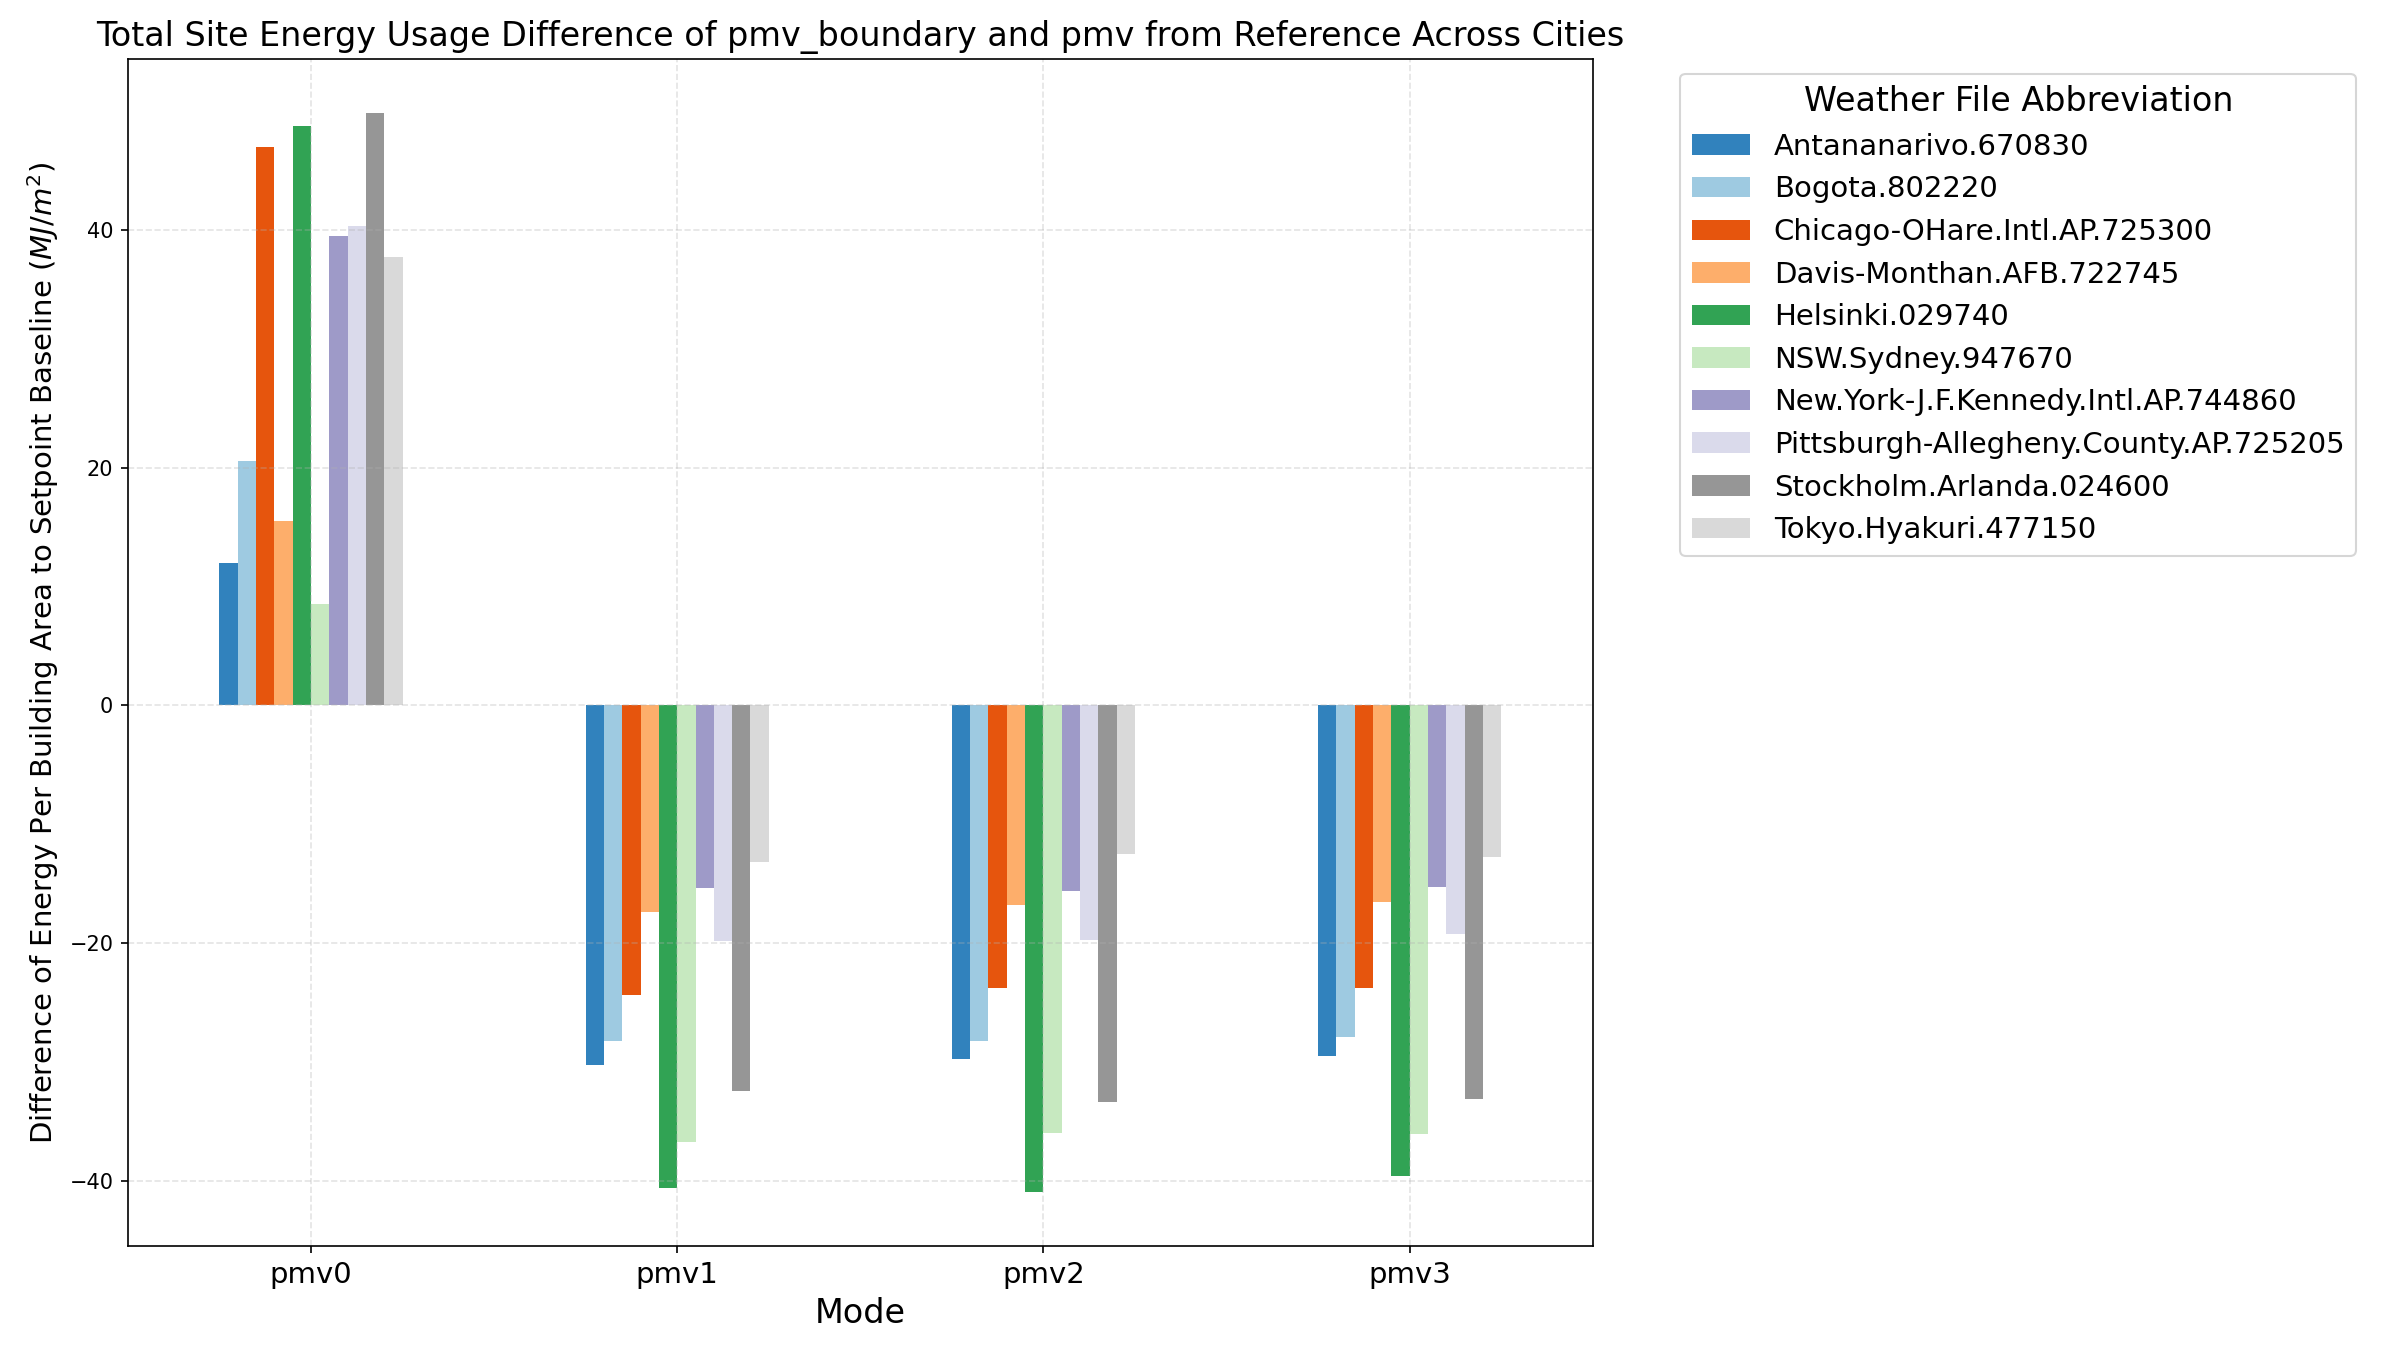
\includegraphics[width=0.85\linewidth]{figs/pmv_search_weather.png}
    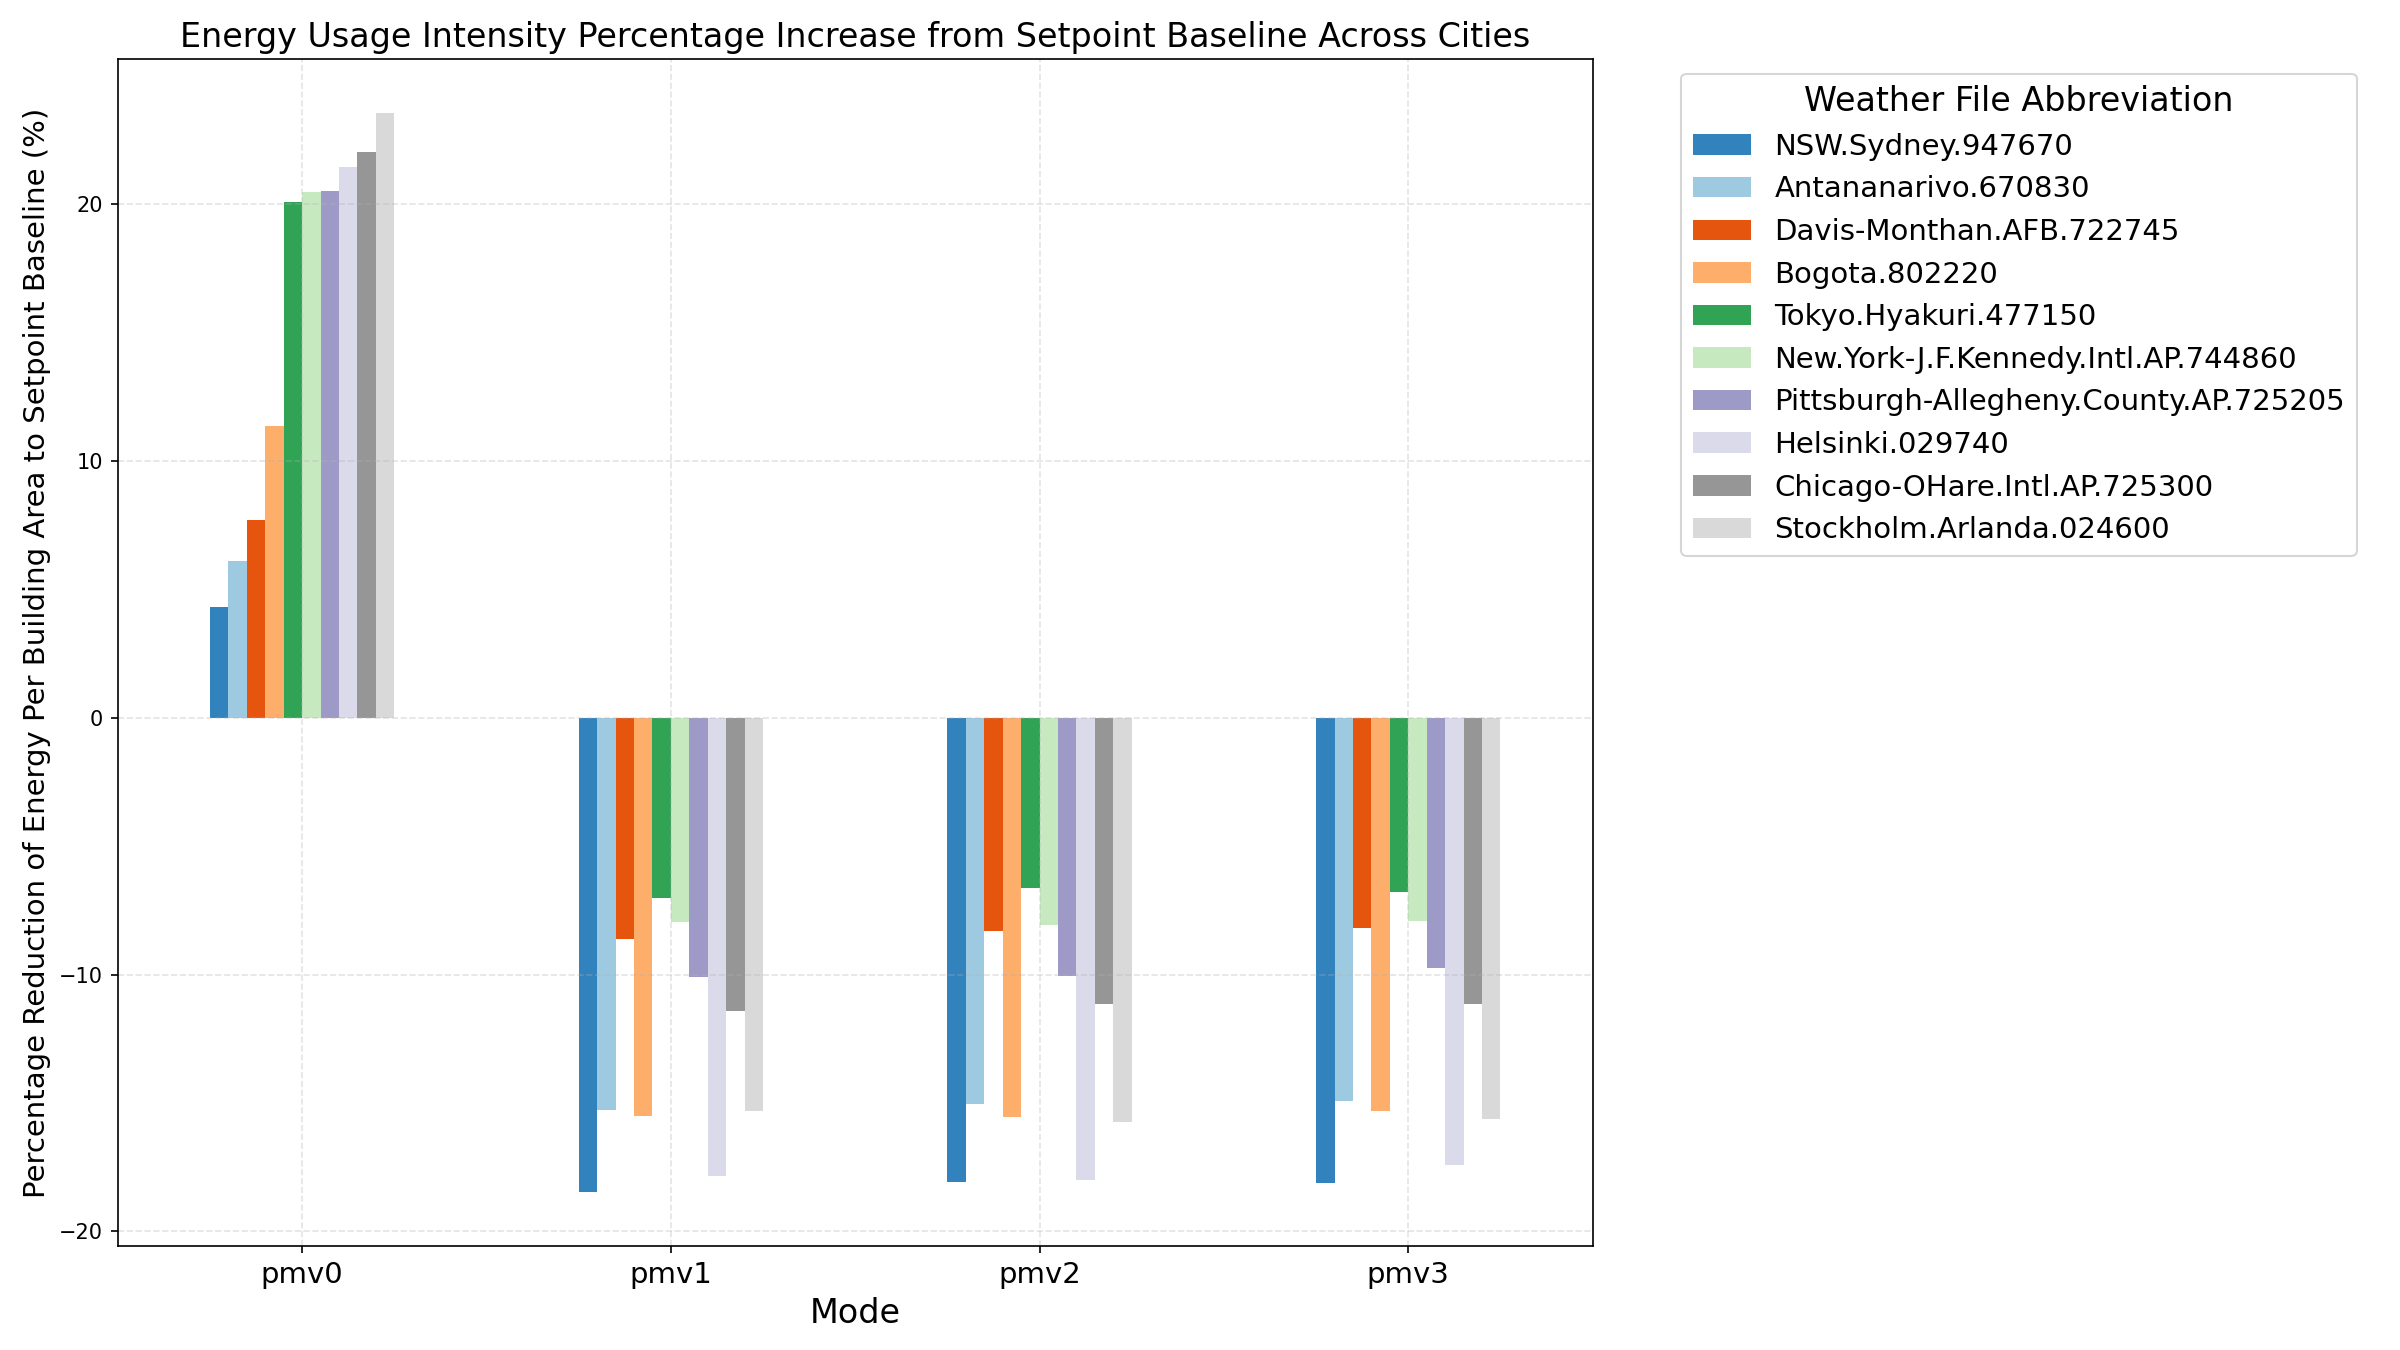
\includegraphics[width=0.85\linewidth]{figs/pmv_search_weather_perc.png}
    \caption{Energy Usage Intensity from EnergyPlus Simulations across multiple weather files (as specified with Figure~\ref{fig:workflow}}
    \label{fig:pmv-grid}
\end{figure}


\subsubsection{Observed Energy Savings with Grid-Search PMV Optimization}

In contrast to \texttt{pmv0}, the PMV-driven strategies employing grid-search optimization (\texttt{pmv1}, \texttt{pmv2}, \texttt{pmv3}), which incorporate different weightings for the energy/comfort trade-off and varied setpoint adjustment step sizes, demonstrated considerable success in reducing energy consumption relative to the bang-bang control.
\paragraph{Significant Savings (approx. 15\% to 18.5\% reduction):} Locations such as Helsinki ($ \approx -17.4\% \text{ to } -18.0\%$), Stockholm ($ \approx -15.3\% \text{ to } -15.8\%$), Sydney ($ \approx -18.1\% \text{ to } -18.5\%$), Bogota ($ \approx -15.3\% \text{ to } -15.6\%$), and Antananarivo ($ \approx -14.9\% \text{ to } -15.3\%$) fall into this category. These results are particularly prominent in climates with substantial heating seasons (Helsinki, Stockholm) but are also evident in the temperate oceanic climate of Sydney and the cooler subtropical highland climates. This suggests that intelligent PMV control can effectively capitalize on opportunities for energy reduction in varied conditions, possibly by optimizing system operation during significant heating/cooling periods or leveraging favorable ambient conditions in milder climates.

\paragraph{Consistent Savings (approx. 7\% to 11.5\% reduction):} Cities like Chicago ($ \approx -11.1\% \text{ to } -11.4\%$), Pittsburgh ($ \approx -9.8\% \text{ to } -10.1\%$), Davis-Monthan AFB ($ \approx -8.2\% \text{ to } -8.6\%$), New York ($ \approx -7.9\% \text{ to } -8.1\%$), and Tokyo ($ \approx -6.7\% \text{ to } -7.0\%$) showed this level of EUI reduction. These savings are observed in continental climates with distinct seasonal swings (Chicago, Pittsburgh, New York) as well as in a hot desert climate (Davis-Monthan) and a humid subtropical one (Tokyo). While the percentage is lower than the first group, the consistency across these demanding climates indicates the broad applicability and benefit of the grid-search PMV approach. Even in cooling-dominated or highly humid environments, these strategies identify pathways to improved efficiency over basic control. 

\begin{figure}[h!]
    \centering
    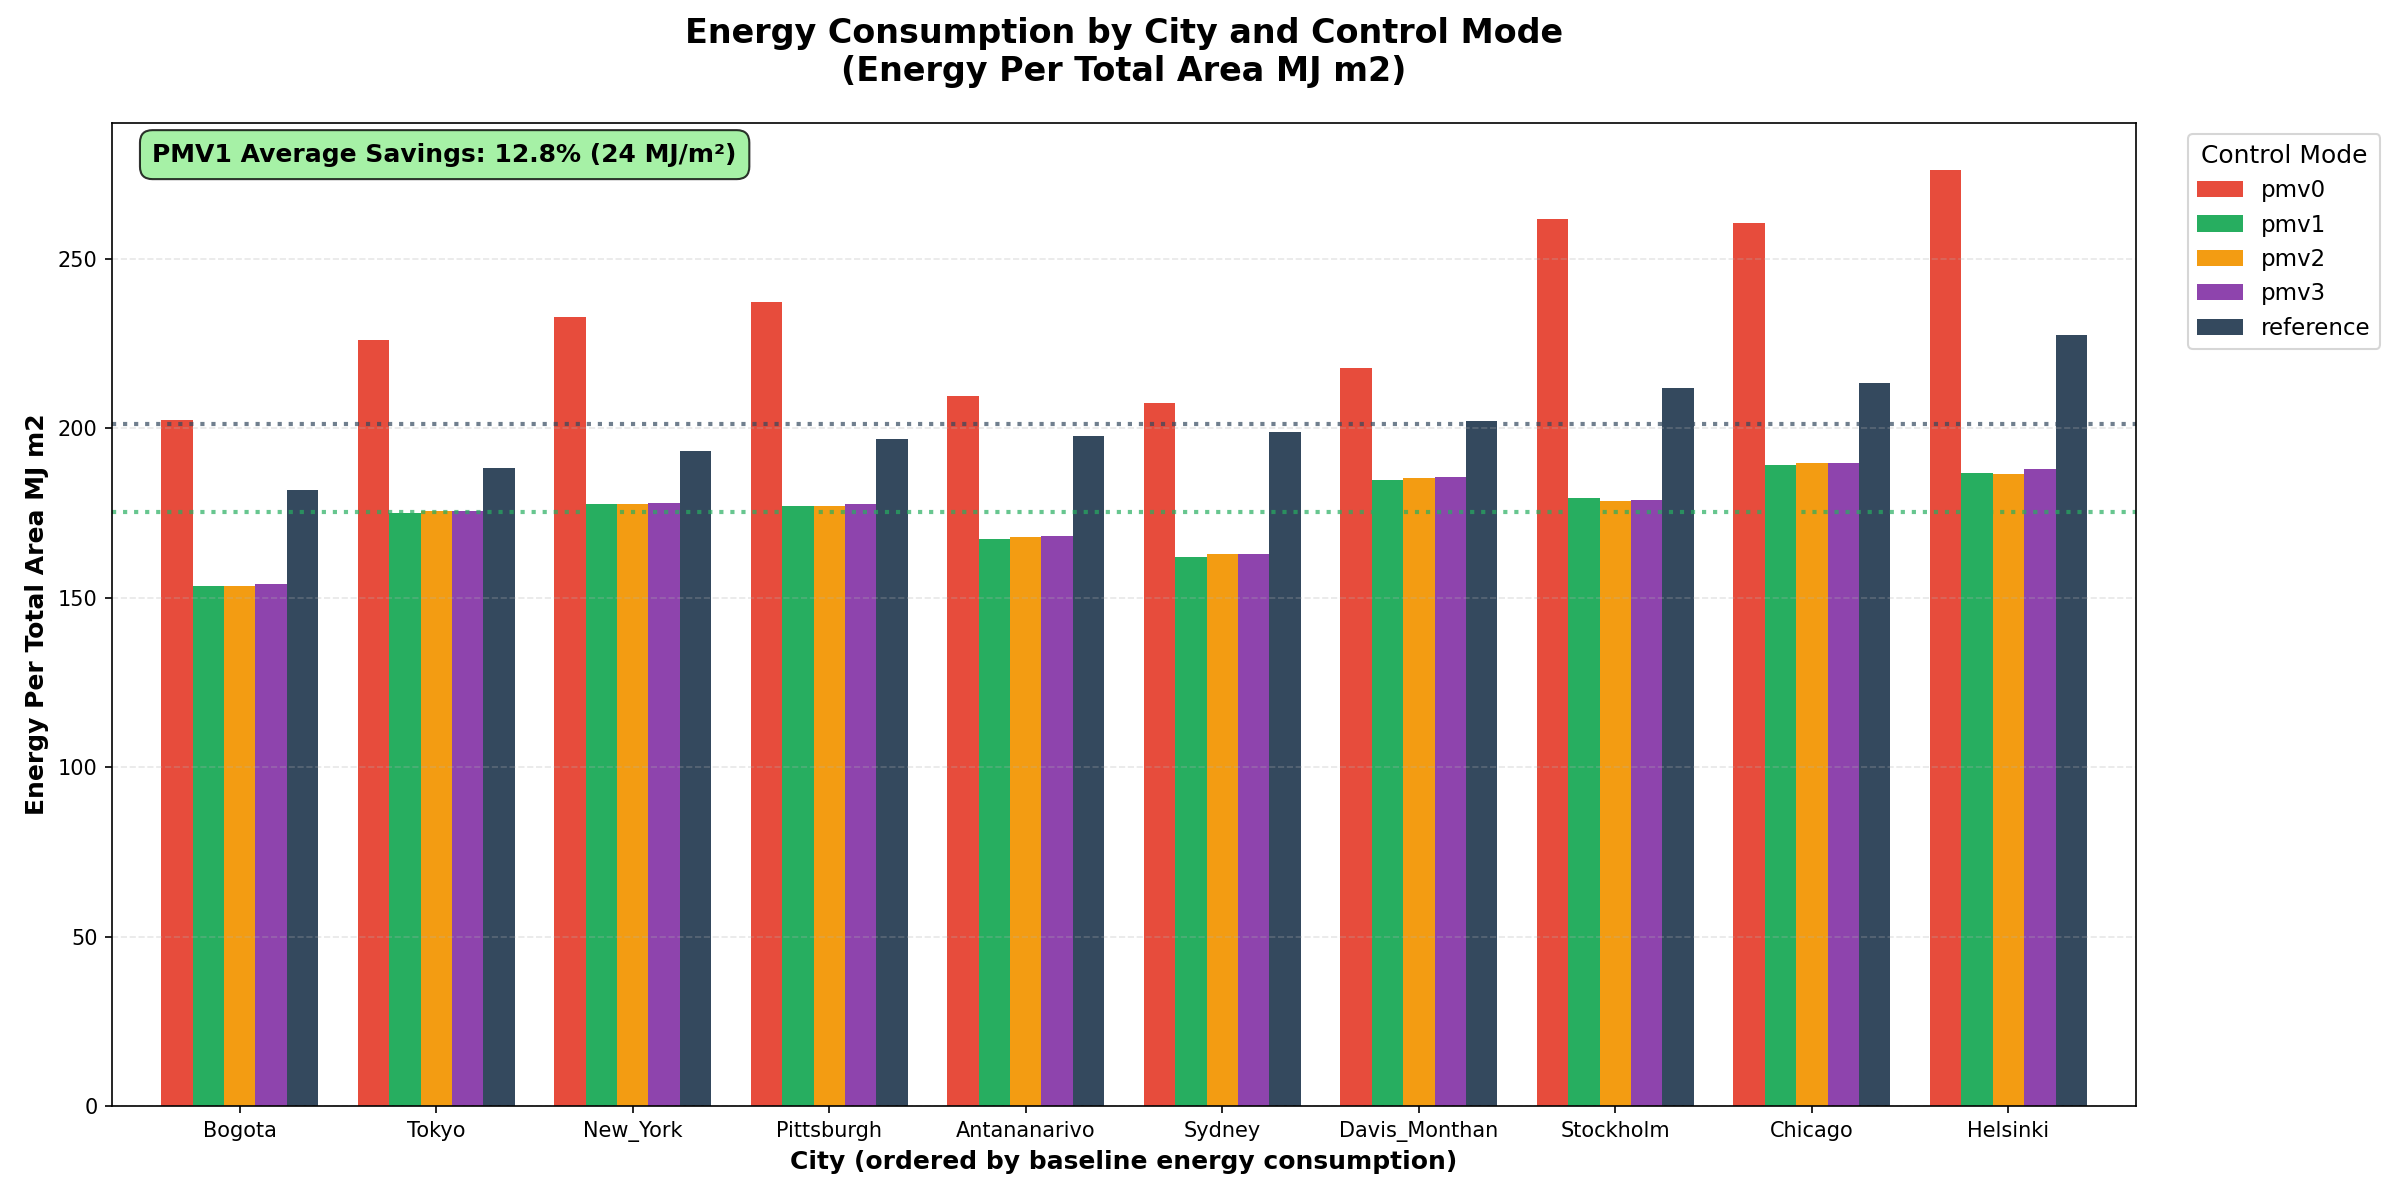
\includegraphics[width=0.95\linewidth]{figs/Energy_Per_Total_Area_MJ_m2_pmv.png}
    \caption{Energy per total area savings across all climates between reference state and all PMV-based control mode variations.}
    \label{fig:MJm2pmv}
\end{figure}

This can be better seen in Figure~\ref{fig:MJm2pmv}, where grid-search approach (\texttt{pmv1}, \texttt{pmv2}, \texttt{pmv3}) is broadly helpful and effective in achieving energy savings. These strategies consistently outperformed both the reference bang-bang control and the simplistic \texttt{pmv0} strategy. Optimized PMV-based control achieved consistent energy savings (averaging at around 12.75\% for PMV1), notably matching ML-based controls. This highlights the unexpected yet robust efficiency achievable by classical comfort models when systematically optimized.

The results clearly highlight that the grid-search approach (pmv1, pmv2, pmv3) is broadly helpful and effective in achieving energy savings. These strategies consistently outperformed both the reference bang-bang control and the simplistic pmv0 strategy. Notably, the three grid-search variants yielded remarkably similar energy savings within each city—typically varying by only one or two percentage points—suggesting that the underlying framework of PMV-based grid search with energy/comfort trade-offs is inherently robust. This convergence in performance indicates there is no single "one-solution-fits-all" strategy among pmv1, pmv2, and pmv3 that consistently yields superior energy results across all diverse climates. While all are effective, the specific parameters (weights, step sizes) explored in these variants might lead to different comfort experiences for occupants, which is not captured in this EUI data but would be a critical consideration for practical implementation. The choice among these similar-performing strategies might ultimately hinge on their differential impact on occupant comfort or other operational considerations beyond pure energy efficiency.

Optimized PMV controls consistently achieved significant (15–18.5\%) or moderate (7–11.5\%) energy savings across diverse climates, demonstrating robust performance independent of geographic and climatic variations. This highlights that grid-search optimization of classical comfort models effectively balances comfort and energy efficiency, rivaling sophisticated ML models.

\subsubsection{Observed Energy Savings with Grid‐Search PMV Optimization}
\label{sec:pmv_energy}

Figure~\ref{fig:stockholm-tokyo} illustrates how the \texttt{pmv1} grid‐search control exploits climatic differences to widen the neutral comfort band. In Stockholm’s cold‐continental summer, lower humidity allows indoor temperatures to reach 27–28\,$^\circ$C (a 5–7\,$^\circ$C expansion from the baseline) without violating PMV neutrality, effectively utilizing `free cooling' from economizer mode operation from June through September. Tokyo's humid-subtropical summer climate restricts this expansion to only 2–3\,$^\circ$C (25–26\,$^\circ$C) due to higher humidity levels that affect thermal comfort. The PMV1 algorithm inherently recognizes these psychrometric constraints and maintains setpoint extremes until indoor conditions approach the boundaries of the expanded comfort range (see Figure~\ref{fig:zoomed-tkst}), resulting in extended economizer mode operation and substantial annual energy reductions without compromising occupant comfort.

\begin{figure}[h!]
    \centering
    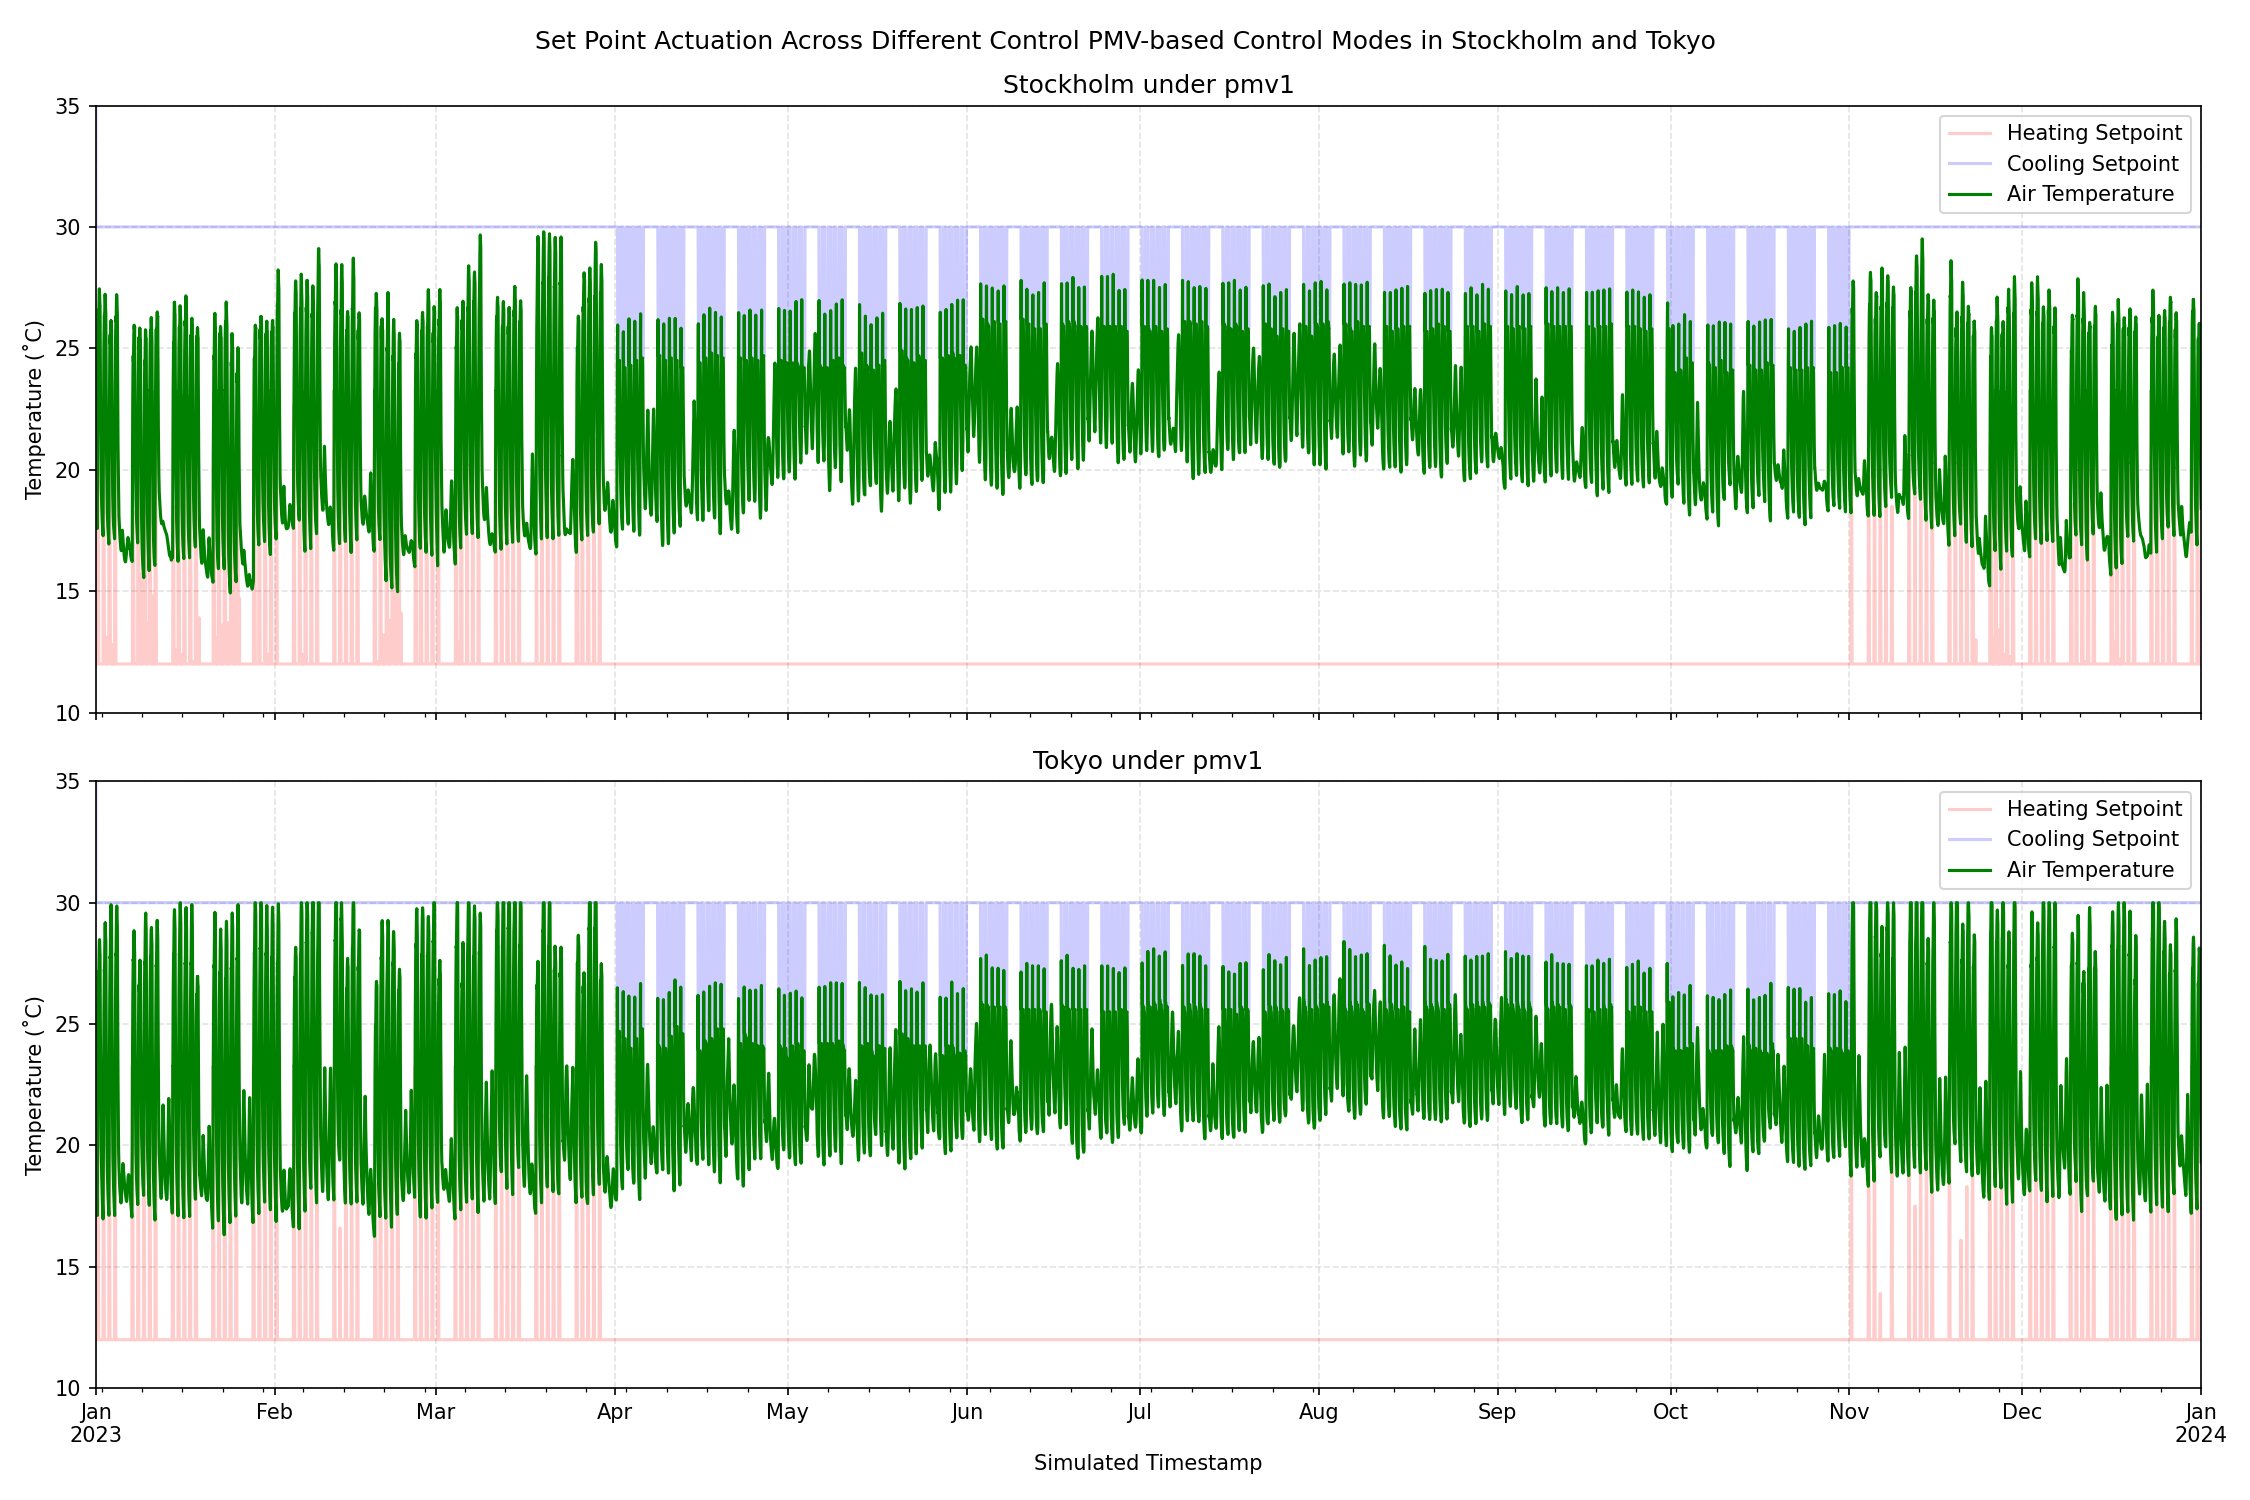
\includegraphics[width=0.95\linewidth]{figs/Stockholm_Tokyo.png}
    \caption{PMV1 control adaptation in contrasting climates: (a) Stockholm’s lower summer humidity permits indoor setpoints of 27–28\,$^\circ$C while maintaining PMV neutrality; (b) Tokyo’s higher humidity constrains summer setpoints to 25–26\,$^\circ$C.}
    \label{fig:stockholm-tokyo}
\end{figure}

\begin{figure}[h!]
    \centering
    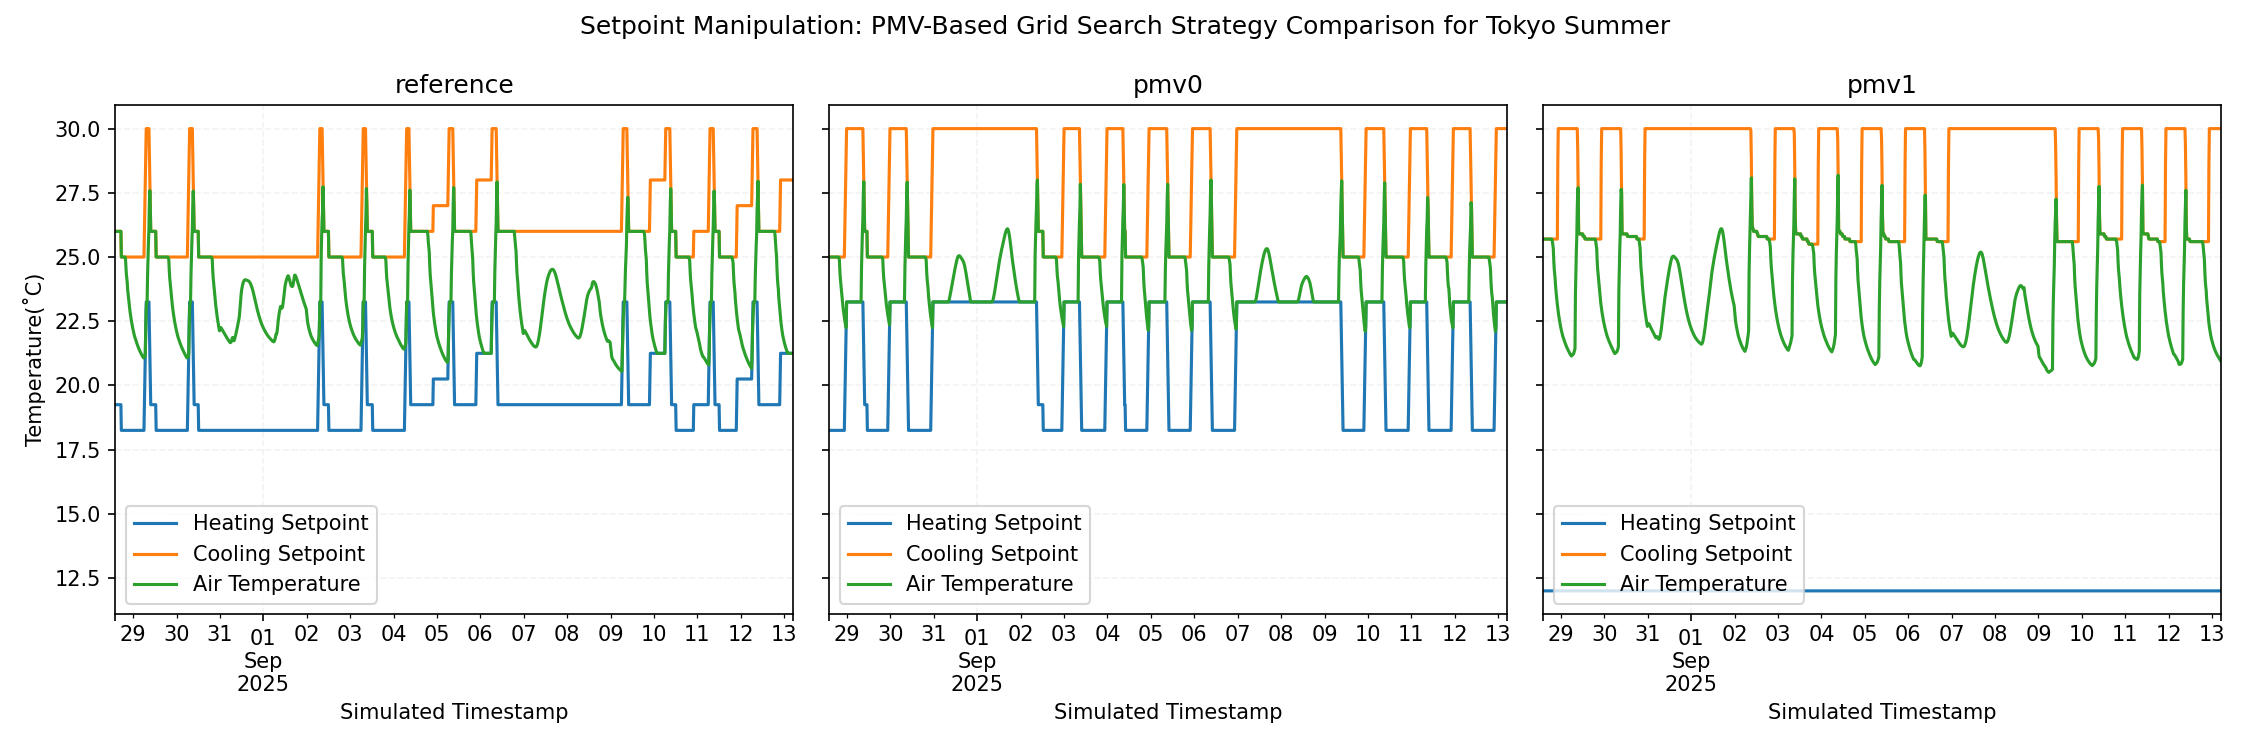
\includegraphics[width=0.75\linewidth]{figs/realcontrol_tk.png}
    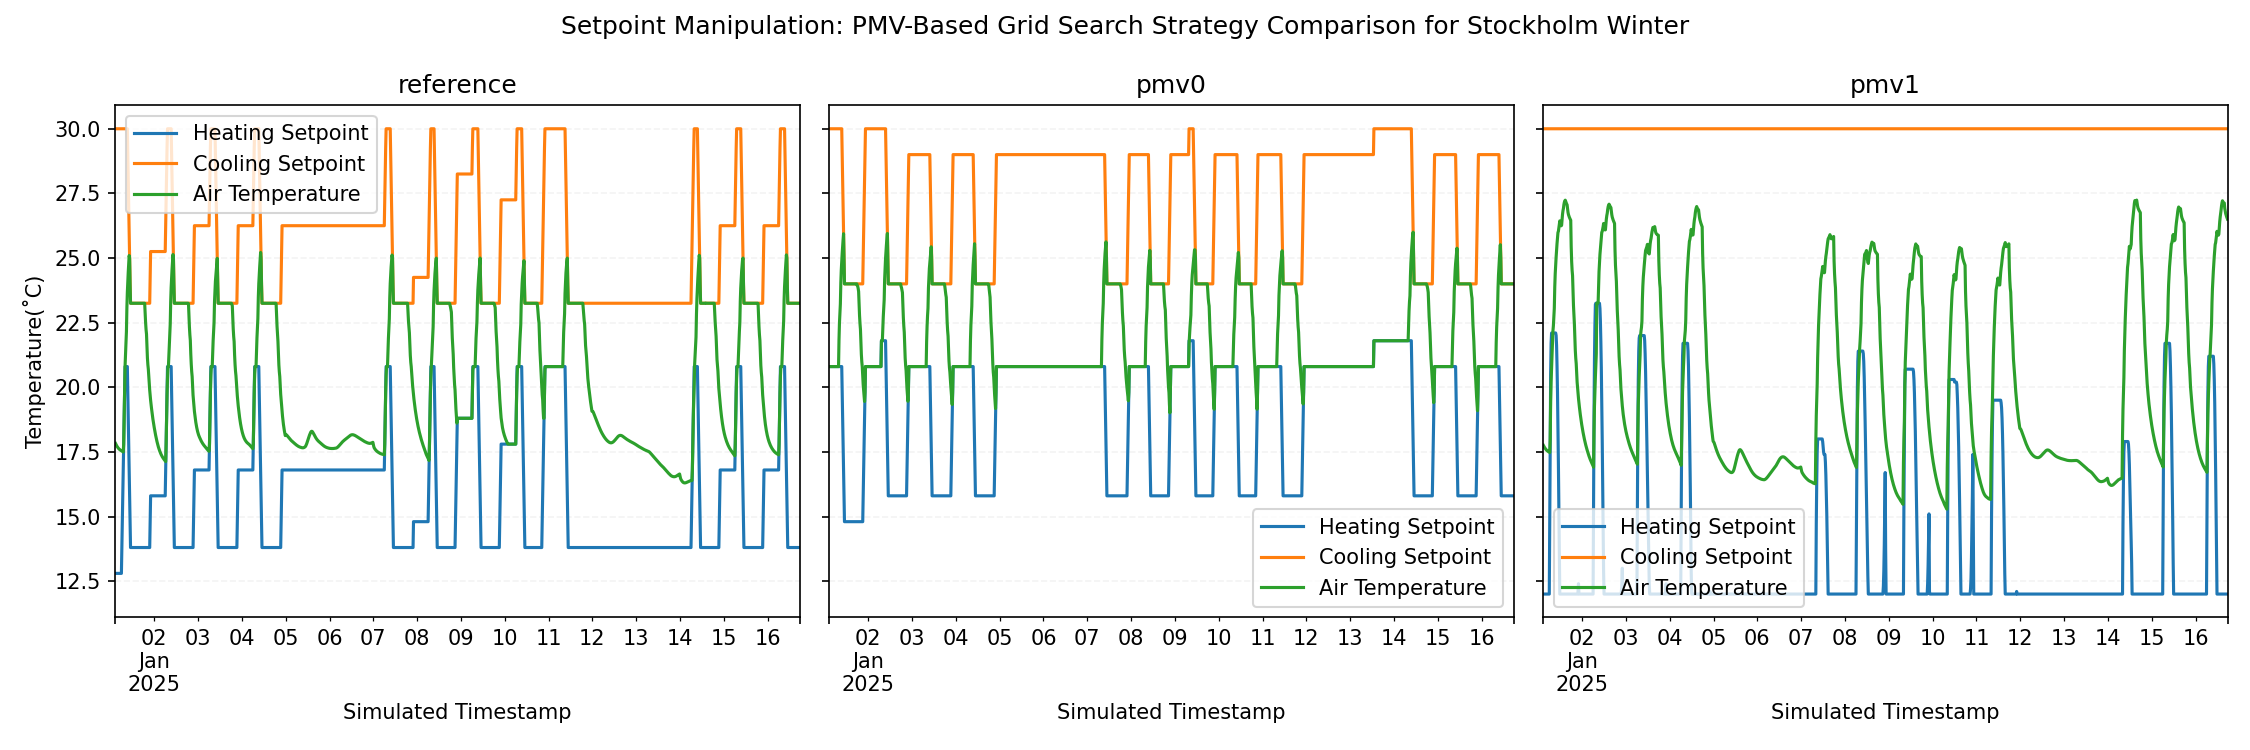
\includegraphics[width=0.75\linewidth]{figs/realcontrol_st.png}
    \caption{Detailed setpoint behavior under PMV1: (top) Tokyo summer holds cooling at the grid‐searched maximum until indoor temperature drifts outside the widened band; (bottom) Stockholm winter holds heating at the minimum as passive gains maintain comfort.}
    \label{fig:zoomed-tkst}
\end{figure}

\subsection{Control Strategy Comparison}
\label{sec:all_control_strategies}
As outlined in the methodology, we compared the seven different control scenarios across four different weather files within our selected IDF file, where we analyze their corresponding energy usage, thermal comfort status, and overall runtime. Figure~\ref{fig:runtime} presents the runtime comparison between the 7 control scenarios. As anticipated, the reference case is consistently the fastest, typically completing annual simulations in 15-20 seconds with no external components to communicate. PMV shows comparable performance at similar runtimes since it's also an analytical model using deterministic calculations. The machine learning models show significantly longer runtimes. LightGBM takes approximately 150-200 seconds per simulation—roughly 10 times slower than reference/PMV—due to model loading and prediction for anticipated occupant arrays. PINN-VAE demonstrates even longer runtimes at 600-900 seconds, as deep learning models require more computational overhead despite vectorized processing.

\begin{figure}[h!]
    \centering
    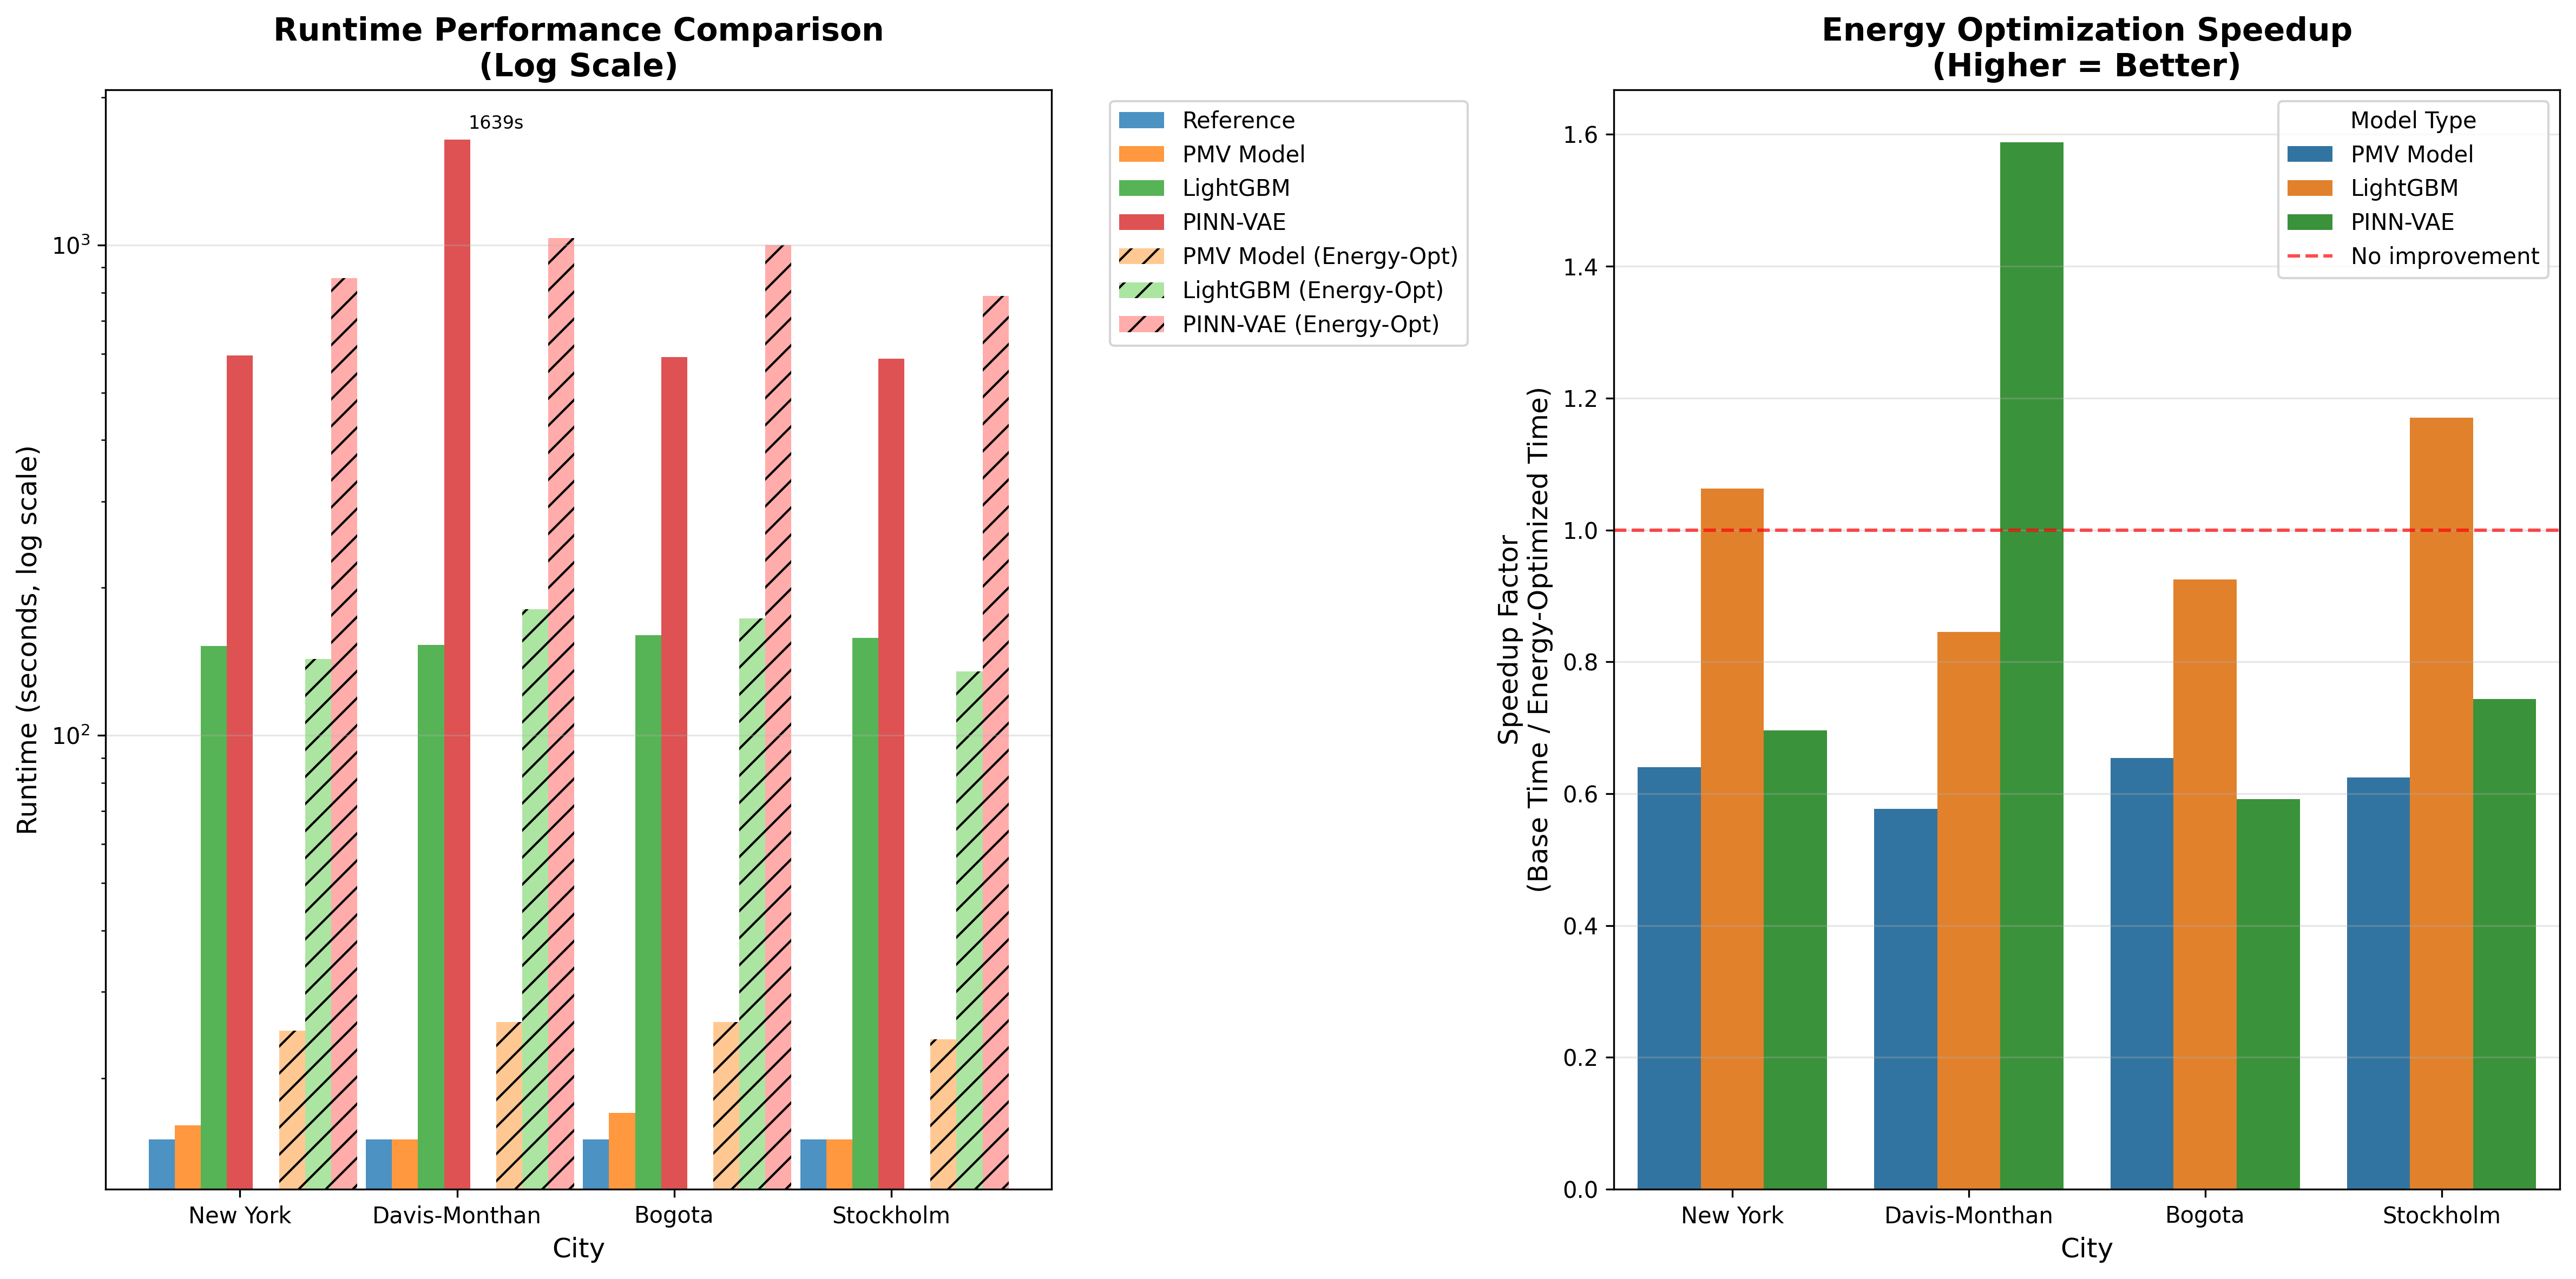
\includegraphics[width=0.75\linewidth]{figs/runtime.png}
    \caption{Runtime comparison between different thermal sensation prediction base models and computational time increase from implicit energy-saving $\Delta T$ grid search.}
    \label{fig:runtime}
\end{figure}

In contrast, the grid search optimization (`-o' variants) reveals interesting patterns: for PMV and LightGBM, the grid search approximately doubles runtime compared to their base versions, reflecting the computational cost of evaluating multiple temperature offset scenarios. However, PINN-VAE shows minimal runtime increase with optimization (comparing `pv' to `pv-o'), suggesting that model inference time dominates over the additional grid search computations. These runtime differences have important implications for real-time control applications, where the sub-200 second performance of optimized PMV and LightGBM remains practical, while PINN-VAE's 10-15 minute runtimes may limit its deployment to offline optimization scenarios.

\subsubsection{Energy Usage and Thermal Comfort Statistics}
\label{sec:energy_comfort_analysis}
This section analyzes the quantitative energy and comfort outcomes of each control strategy, examining total consumption, component-level breakdowns, and thermal comfort distributions.
We first examine the energy and comfort performance of each control strategy. Figure~\ref{fig:energy_ranking} presents the annual energy consumption ranking (1 = most efficient) for each control mode in Bogota, Davis‐Monthan, New York, and Stockholm. Across all four climates, the optimized grid‐search variants (\texttt{pmv-o}, \texttt{lightgbm-o}, \texttt{pv-o}) consistently occupy the top three positions, demonstrating robust, climate‐independent performance. In contrast, the “pure” modes (\texttt{pmv}, \texttt{lightgbm}, \texttt{pv}) occupy the lower ranks (5–7), despite sometimes achieving localized cooling or fan energy reductions. This discrepancy arises because unoptimized controllers frequently request setpoints beyond the 12 $^\circ$C–30 $^\circ$C limits, leading to actuator clipping and spurious energy savings in one end use that are more than offset by large energy penalties in another. The baseline \texttt{reference} (`bang–bang') control invariably sits in the middle (rank 4), underscoring that naïve comfort‐based inversions can underperform a simple hysteresis thermostat when actuator saturation is not considered.

\begin{figure}[h!]
    \centering
    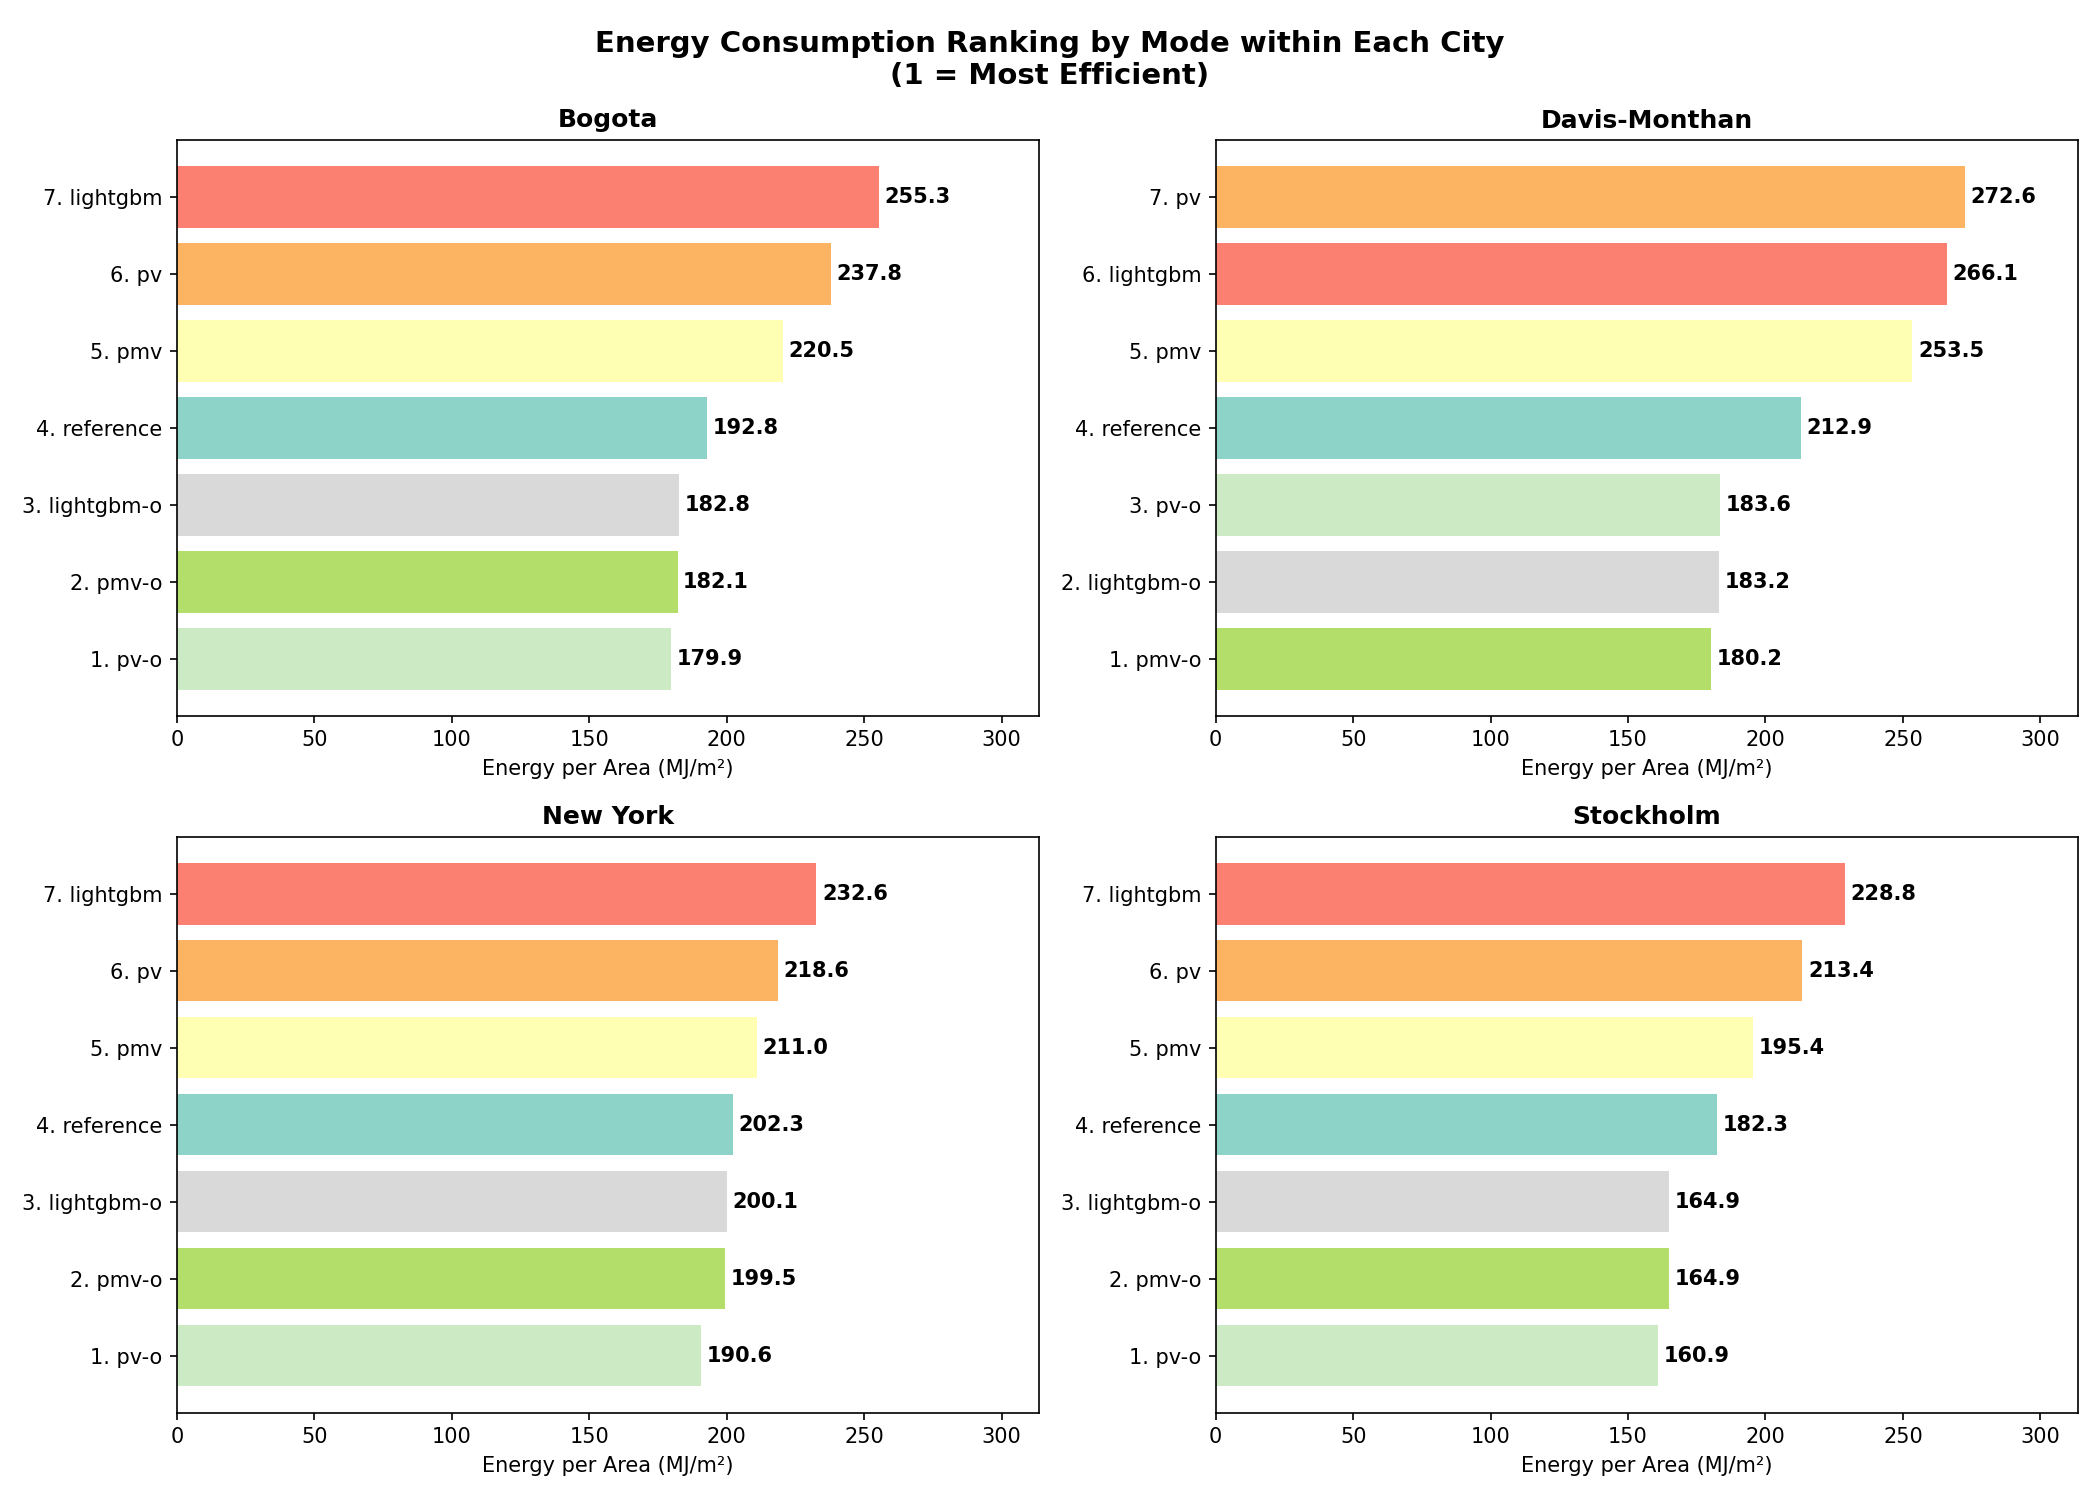
\includegraphics[width=\linewidth]{figs/energy_consumption_ranking_by_mode_within_each_city.png}
    \caption{Energy consumption ranking (1 = most efficient) for each control mode in four cities. Grid‐search variants (\texttt{pmv-o}, \texttt{lightgbm-o}, \texttt{pv-o}) occupy the top three ranks, while unoptimized “pure” modes (\texttt{pmv}, \texttt{pv}, \texttt{lightgbm}) lie at the bottom.}
    \label{fig:energy_ranking}
\end{figure}

Figure~\ref{fig:thermal_comfort} compares thermal comfort (Predicted Mean Vote, PMV) and indoor temperature distributions across all seven modes in the same four cities. The grid‐search variants maintain median PMV values tightly within the neutral band (–0.5 to +0.5) and exhibit markedly smaller interquartile ranges than the pure modes. For example, \texttt{pv-o} and \texttt{pmv-o} rarely exceed $\pm$0.5, indicating consistent comfort despite varying external conditions. By contrast, \texttt{lightgbm} and \texttt{pv} without optimization show bimodal PMV distributions, with frequent excursions above +1.0 or below –1.0, reflecting repeated setpoint clipping at 12$^\circ$C or 30$^\circ$C. These clipping‐induced comfort violations correspond to the oscillatory indoor temperature patterns visible in the lower panel: the pure ML/PV modes force indoor air to swing between the extremes of 12$^\circ$C and 30$^\circ$C, whereas grid‐search controllers keep most of their temperatures in the 22–26$^\circ$C range. This stabilization of indoor conditions not only preserves occupant comfort but also eliminates the energy wasted on cycling between extremes.

\begin{figure}[h!]
    \centering
    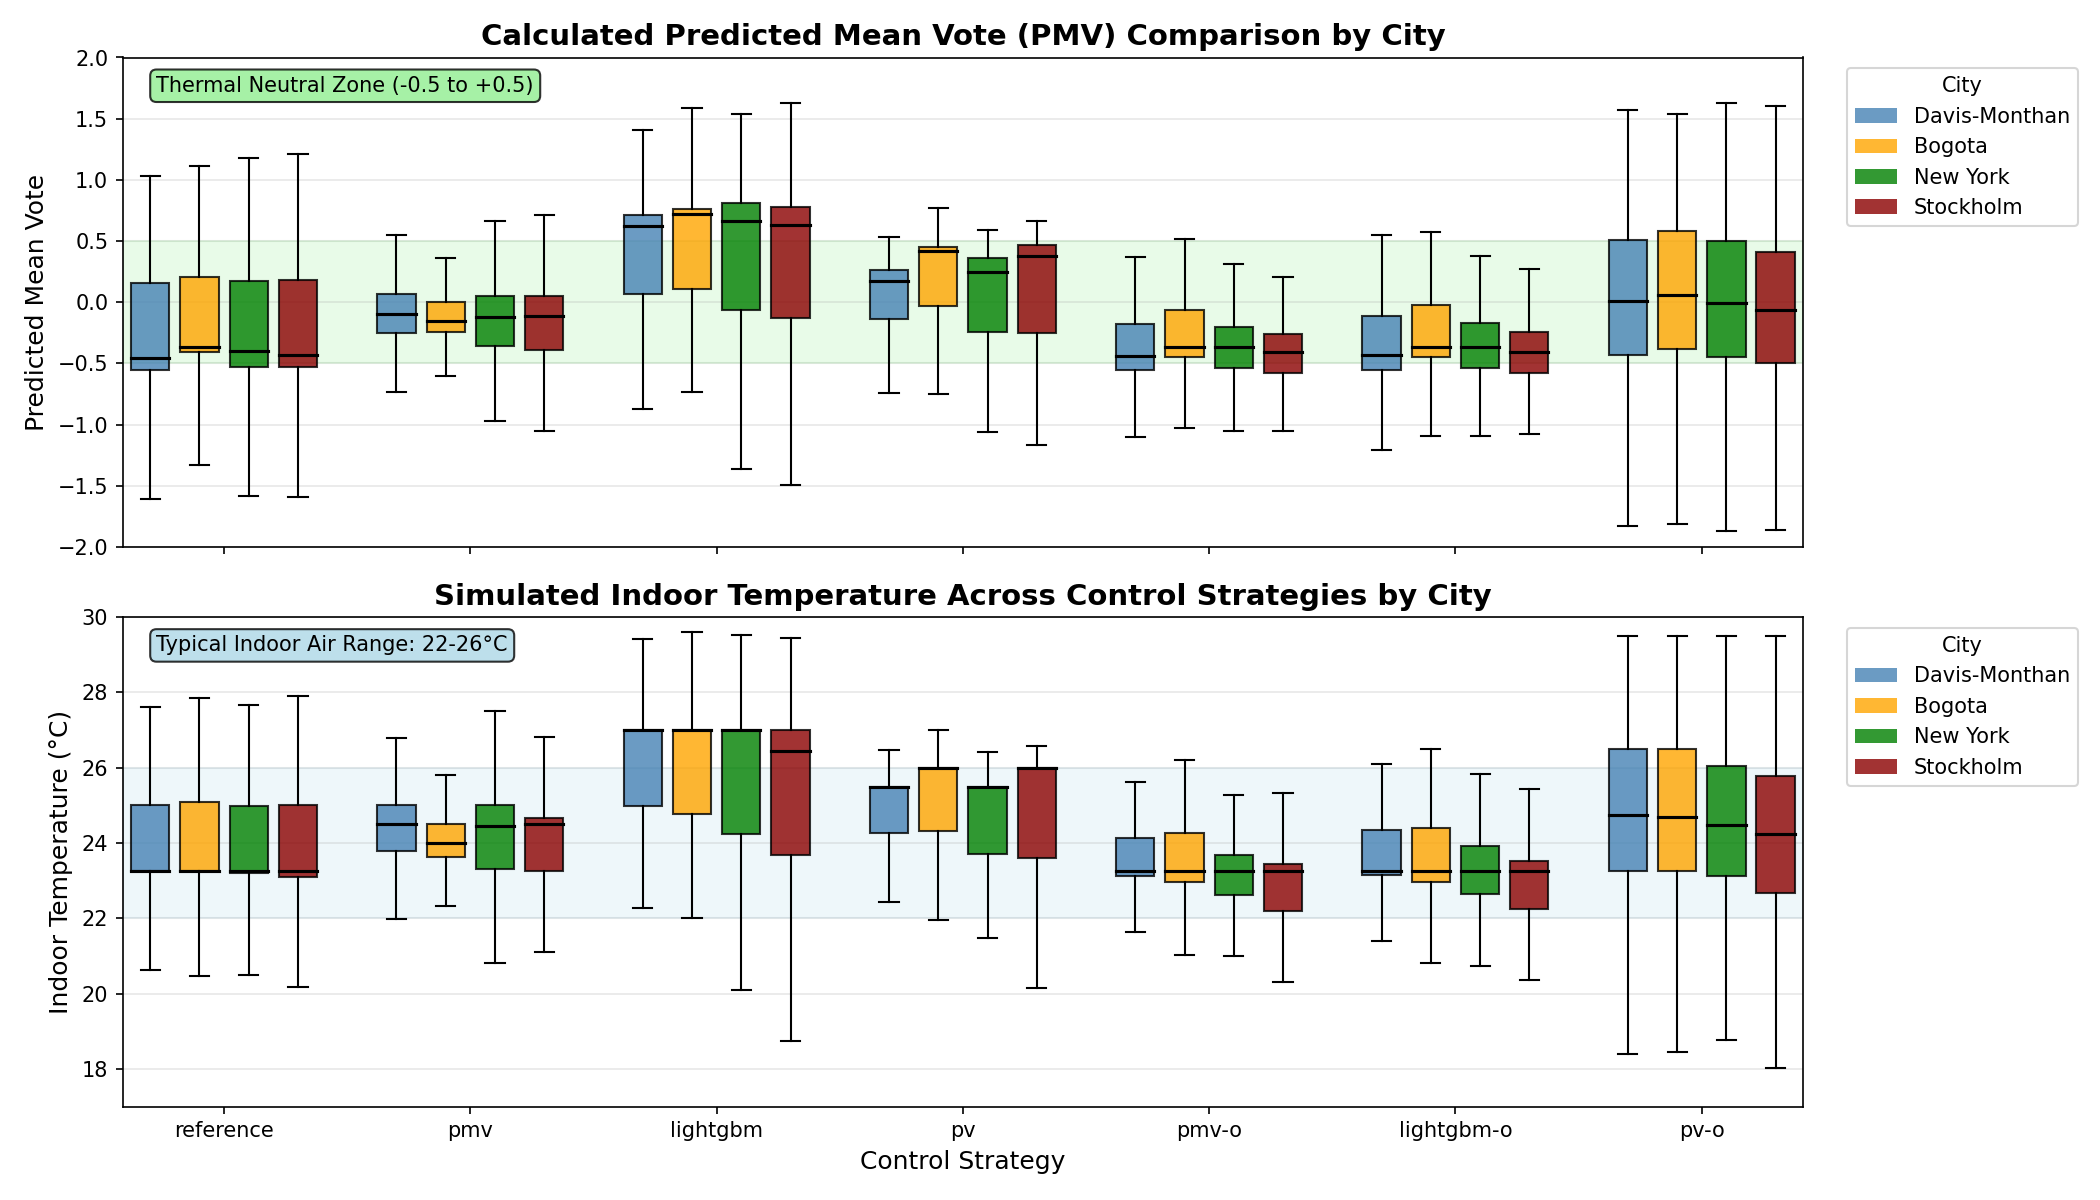
\includegraphics[width=\linewidth]{figs/thermal_comfort_comparison_improved.png}
    \caption{Top: PMV distributions by control mode and city (green shading = comfort zone, $\pm$0.5). Bottom: Indoor temperature distributions (blue shading = typical comfort range, 22–26$^\circ$C). Grid‐search variants exhibit tighter comfort control and avoid clipping‐induced extremes.}
    \label{fig:thermal_comfort}
\end{figure}

Figure~\ref{fig:component_savings} breaks down energy savings (relative to \texttt{reference}) into heating, cooling, and fan components for each city. The grid‐search PMV variant (\texttt{pmv-o}) achieves the largest heating reductions—up to +91\% in Bogota and +79\% in Davis—by tolerating expanded neutral temperature bands in summer and leveraging passive gains in winter. Although \texttt{pmv-o} incurs small negative cooling savings in colder climates (e.g., –16\% in Stockholm), the net effect is still a substantial reduction in overall HVAC energy. Similarly, \texttt{lightgbm-o} and \texttt{pv-o} realize significant heating savings (+58\% to +75\%) with modest cooling trade‐offs. In contrast, the unoptimized \texttt{lightgbm} and \texttt{pv} modes display large negative heating “savings”—for instance, –889\% in Davis and –295\% in New York—because they remain pinned at 12$^\circ$C during extremes and then must repeatedly reheat, creating enormous energy penalties. Their apparent cooling or fan energy gains are insufficient to offset these heating losses, confirming that actuator clipping can produce misleading component‐level metrics.

\begin{figure}[h!]
    \centering
    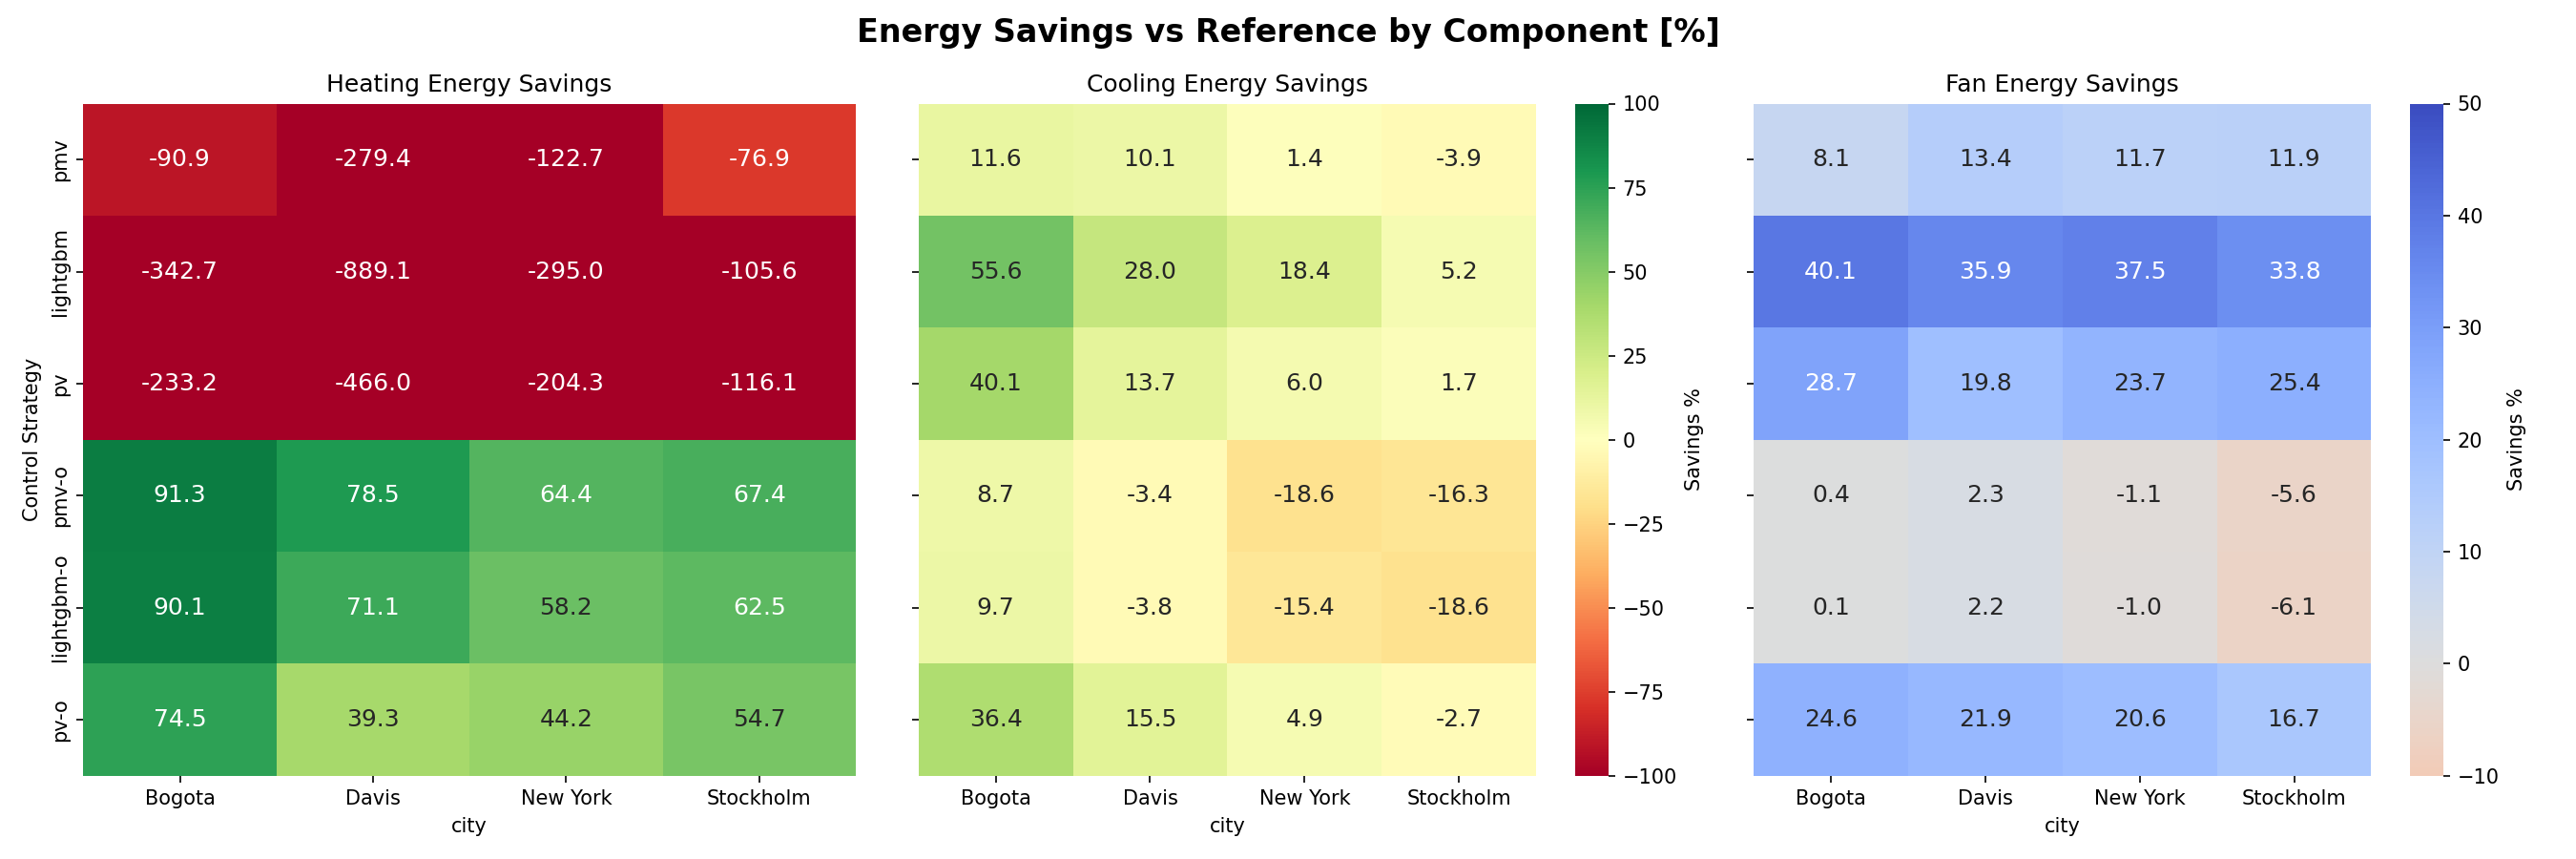
\includegraphics[width=\linewidth]{figs/saving_end_pct.png}
    \caption{Component‐level energy savings (\%) relative to \texttt{reference}, by city and control mode. Positive values indicate reduced consumption. Grid‐search variants (\texttt{pmv-o}, \texttt{lightgbm-o}, \texttt{pv-o}) achieve large heating savings with minor cooling/fan trade‐offs, while pure modes incur large heating penalties due to clipping.}
    \label{fig:component_savings}
\end{figure}

When aggregated into total HVAC energy savings (Figure~\ref{fig:hvac_savings}), grid‐search variants consistently deliver substantial net reductions—from 90\% in Bogota to 62\% in Stockholm—highlighting the method’s ability to achieve “win–win” outcomes: maintaining neutral PMV and stable indoor temperatures while dramatically lowering energy use. In contrast, pure \texttt{lightgbm} and \texttt{pv} modes produce negative net savings across all climates (e.g., –466\% in Davis, –204\% in New York), reflecting their pathological reliance on setpoints clipped to extremes. The \texttt{reference} controller (0\% savings by definition) outperforms unoptimized pure modes in some climates, underscoring that a simplistic hysteresis thermostat can surpass naïve comfort‐driven logic when actuator saturation is unresolved.

\begin{figure}[h!]
    \centering
    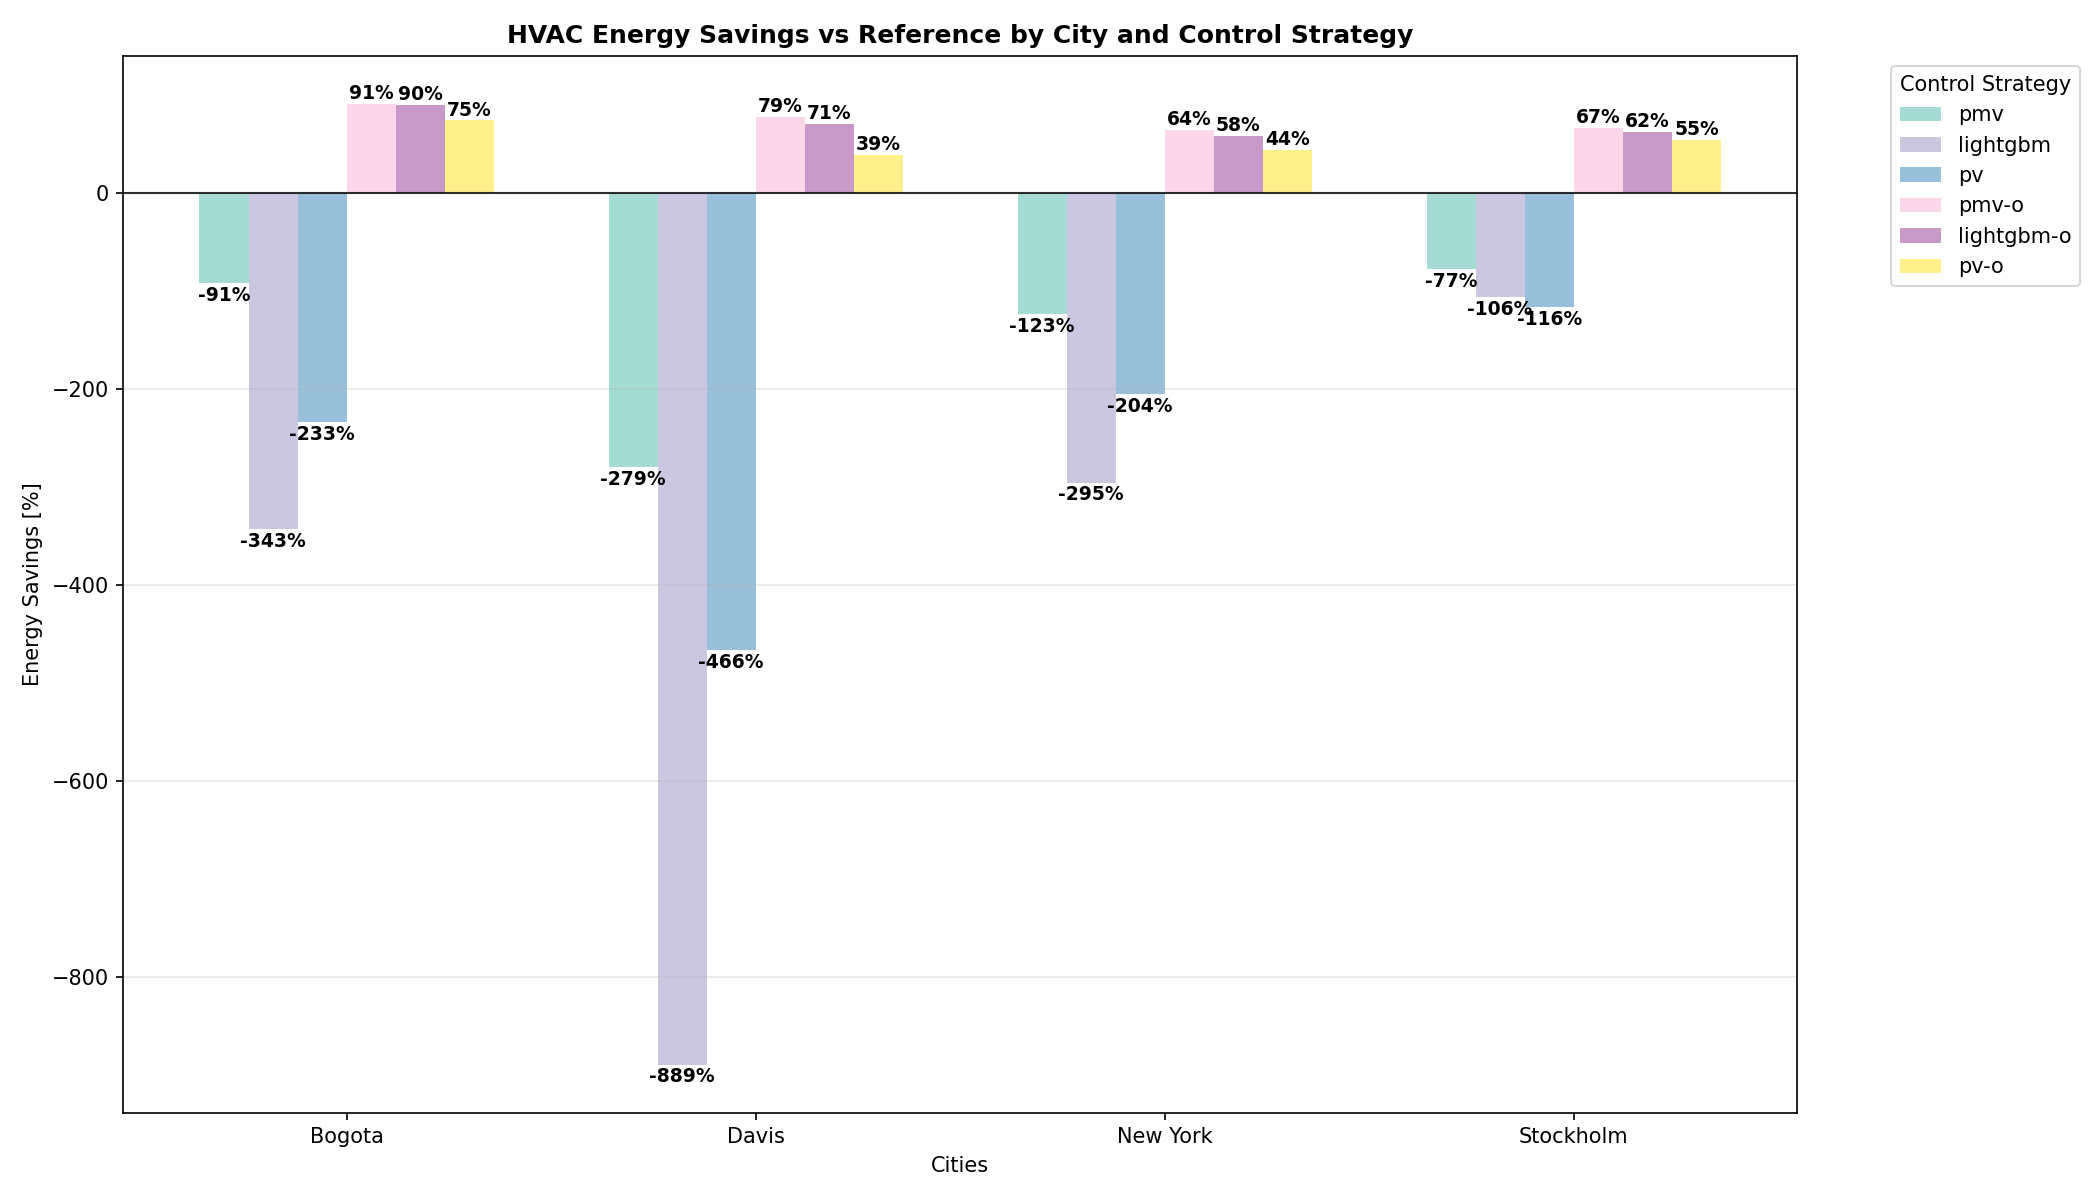
\includegraphics[width=\linewidth]{figs/savings_r.png}
    \caption{Total HVAC energy savings (\%) relative to \texttt{reference} across four cities. Grid‐search variants (\texttt{pmv-o}, \texttt{lightgbm-o}, \texttt{pv-o}) yield 62\%–90\% savings; unoptimized modes incur large negative savings due to actuator clipping.}
    \label{fig:hvac_savings}
\end{figure}


\subsubsection{Performance Hierarchy and Climate Consistency Analysis}
\label{sec:performance_hierarchy}
Having established the performance metrics, we now examine how these rankings remain consistent across diverse climates. 
As shown in Figure~\ref{fig:energy_ranking}, annual energy consumption (MJ/m²) for each control mode in Bogota, Davis‐Monthan, New York, and Stockholm (1 = most efficient) are plotted and ranked accordingly. Across all four climates, the optimized grid‐search variants (\texttt{pv-o}, \texttt{pmv-o}, \texttt{lightgbm-o}) occupy the top three positions, with \texttt{pv-o} and \texttt{pmv-o} typically tied for first or second. The baseline \texttt{reference} control consistently falls in the middle (rank 4), while the unoptimized “pure” modes (\texttt{pmv}, \texttt{pv}, \texttt{lightgbm}) occupy ranks 5–7, reflecting their inability to avoid actuator saturation.

While the previous section showed absolute performance differences, here we observe that climate-specific nuances appear primarily among the mid-rank and bottom modes, with top performers maintaining their advantage regardless of location. In Bogota and New York, \texttt{lightgbm-o} edges out \texttt{pmv-o} by a small margin, whereas in Davis‐Monthan and Stockholm, \texttt{pmv-o} ties or slightly outperforms \texttt{pv-o}. Among the unoptimized controllers, \texttt{pmv} often ranks lower in cold climates (Stockholm) but improves modestly in mixed or hot climates (Bogota, Davis‐Monthan). Similarly, \texttt{lightgbm} and \texttt{pv} without grid optimization display high variability—\texttt{lightgbm} fares better in New York but poorly in Davis‐Monthan, while \texttt{pv} consistently remains mid‐tier. Overall, the grid‐search optimization engenders both superior and more climate‐robust performance, demonstrating that a properly tuned analytical or ML‐based method consistently outperforms unoptimized strategies across diverse thermal conditions.


\subsubsection{Actuator Saturation Analysis}
\label{sec:actuator_saturation_results}
Our co-simulation methodology enables direct observation of actuator saturation behavior—a critical deployment challenge that pure comfort prediction research often overlooks. This phenomenon occurs when a controller's requested heating setpoint falls below the hard minimum ($12\,^\circ\mathrm{C}$) or its requested cooling setpoint exceeds the hard maximum ($30\,^\circ\mathrm{C}$). 
EnergyPlus (via Sinergym) then clips the setpoint to that boundary; further commands in the same direction have no effect. Table~\ref{tab:saturation_rates} demonstrates our framework's capability to quantify this saturation behavior, reporting the percentage of occupied hours during which each controller was clipped to 12 $\degree C$ or 30 $\degree C$ under both original and boundary-optimized implementations.

\begin{table}[!]
  \centering
  \caption{Percentage of occupied hours clipped to actuator bounds, before vs.\ after boundary optimization.}
  \label{tab:saturation_rates}
  \resizebox{\textwidth}{!}{
  \begin{tabular}{l|rrrrrr}
    \toprule
    \multirow{2}{*}{Controller Mode} & \multicolumn{3}{c}{Before} & \multicolumn{3}{c}{After} \\
    \cmidrule(lr){2-4} \cmidrule(lr){5-7}
    & \% @ 12~$^\circ$C & \% @ 30~$^\circ$C & \% Total Clipped
    & \% @ 12~$^\circ$C & \% @ 30~$^\circ$C & \% Total Clipped \\
    \midrule
    reference              & $0.00\%$ & $2.84\%$ & $2.84\%$ & $0.00\%$ & $2.85\%$ & $2.85\%$ \\
    PMV (pure)             & $0.00\%$ & $13.99\%$ & $13.99\%$ & $0.00\%$ & $0.10\%$ & $0.10\%$ \\
    LightGBM (pure)        & $4.52\%$ & $7.95\%$ & $7.95\%$ & $0.00\%$ & $4.52\%$ & $4.52\%$ \\
    PV (pure)              & $0.00\%$ & $0.39\%$ & $0.39\%$ & $0.00\%$ & $0.12\%$ & $0.12\%$ \\
    PMV-o (grid-search)    & $0.02\%$ & $66.95\%$ & $66.95\%$ & $0.00\%$ & $32.70\%$ & $32.70\%$ \\
    LightGBM-o (grid-search)& $0.00\%$ & $73.82\%$ & $73.82\%$ & $0.00\%$ & $32.70\%$ & $32.70\%$ \\
    PV-o (grid-search)     & $0.14\%$ & $67.76\%$ & $67.76\%$ & $0.00\%$ & $33.45\%$ & $33.45\%$ \\
    \bottomrule
  \end{tabular}
  }
\end{table}

Examining results from Table~\ref{tab:saturation_rates}, we could quickly come to the following key observations:
\begin{itemize}
  \item \textbf{Heating‐side saturation is eliminated after boundary optimization.} All controllers show $0.00\%$ clipped at $12\,^\circ\mathrm{C}$ in the ``After'' columns, confirming that the $\pm2\,^\circ\mathrm{C}$ grid around the interior reset prevents any candidate from falling below $12\,^\circ\mathrm{C}$.  
  \item \textbf{Cooling‐side saturation remains substantial.}  Even after boundary optimization, PMV‐o, LightGBM‐o, and PV‐o clip at $30\,^\circ\mathrm{C}$ approximately one‐third of occupied hours (32.70–33.45\%). This indicates that under hot conditions, all $\Delta T$ candidates eventually hit the hard ceiling, and the controller remains pinned until comfort can be restored by other means.  
  \item \textbf{Pure ML/PV controllers improve heating saturation but still clip on cooling.}  LightGBM (pure) goes from $4.52\%$ clipped at $12\,^\circ\mathrm{C}$ “Before” to $0.00\%$ “After,” but still clips at $30\,^\circ\mathrm{C}$ for $4.52\%$ of occupied hours. PV (pure) clips at $30\,^\circ\mathrm{C}$ for only $0.12\%$ “After,” down from $0.39\%$.  
  \item \textbf{Complete elimination of cooling saturation is unrealistic.}  In very hot climates or during periods of peak internal gains, any controller will at times demand a cooling setpoint below $30\,^\circ\mathrm{C}$. Because EnergyPlus enforces the $30\,^\circ\mathrm{C}$ ceiling, saturation at that limit is inevitable whenever comfort cannot be maintained otherwise.  
  \item \textbf{Value of the ``Before vs.\ After'' comparison.}  Reporting both sets of numbers reveals how boundary optimization transforms LightGBM (pure) and PV (pure) from pathological “always‐clipped” strategies into far more balanced approaches. For instance, LightGBM (pure) used to clip at $12\,^\circ\mathrm{C}$ for $4.52\%$ of hours, but LightGBM‐o never clips at $12\,^\circ\mathrm{C}$—instead, it only clips at $30\,^\circ\mathrm{C}$ for $32.70\%$ of hours, reflecting honest, interior comfort attempts.  
\end{itemize}
\noindent

These results have practical implication for future controller design, particularly when co-simulating with Machine-Learning-based control log. Any ML‐based or DL‐based control logic that does not explicitly account for these hard actuator bounds will likely exhibit high saturation rates and derive spurious energy‐comfort conclusions. Our boundary‐optimized grid search successfully removes “too‐cold” saturation entirely and reduces “too‐hot” saturation by roughly half. Further improvements may involve predictive models (e.g., Model Predictive Control), anti‐windup PIDs, or RL agents with an explicit clipping penalty to minimize residual saturation under extreme conditions.  

\subsection{Incorporation of Physiological Variables into Control Strategy}
\label{sec:tsk_results}
As outlined in Section~\ref{sec:pv_tsk_control}, two $T_{skin}$ incorporated control strategies based on boundary-optimized PINN-VAE strategy are further applied to the simulation experiments with the results shown in Table~\ref{tab:pv_tsk_results}. \texttt{pv-tsk-strict} strategy demonstrates a notable improvement in comfort evaluation (15.10\% on average) compared to \texttt{pv-o}, accompanied by a slight increase in energy consumption (1.97\% on average) while the \texttt{pv-tsk-loose} mode shows negligible differences.

\begin{table}[htbp]
\begin{center}
\small
\caption{Percentage Change in EUI and Uncomfort Hour (Simple ASHRAE 55-2004) for $T_{skin}$-involved Strategies Compared to \texttt{pv-o}}
\label{tab:pv_tsk_results}
\vspace{0.5em}
\setlength{\tabcolsep}{6pt} % Adjust spacing between columns
\begin{tabular}{lcc|cc}
\toprule
\makecell[l]{City/\\Site} 
& \multicolumn{2}{c|}{pv-tsk-strict} 
& \multicolumn{2}{c}{pv-tsk-loose} \\
\cmidrule(lr){2-3} \cmidrule(lr){4-5}
& EUI(\%) & Uncomfort Hour(\%) & EUI(\%) & Uncomfort Hour(\%) \\
\midrule
Bogota        & $1.90$ & $-11.83$ & $0.10$ & $-0.20$ \\
Stockholm     & $0.85$ & $-18.36$ & $-0.71$ & $1.33$ \\
Davis-Monthan & $2.30$ & $-11.65$ & $0.10$ & $0.04$  \\
New York      & $2.85$ & $-18.57$ & $0.14$ & $0.08$  \\
\midrule
Average       & $1.97$ & $-15.10$ & $-0.09$ & $0.32$ \\
\bottomrule
\end{tabular}
\vspace{0.5em} \\
\footnotesize
\textit{Note:} Negative values signify a decrease in EUI (energy savings) and uncomfort hour (comfort improvement).
\end{center}
\end{table}

We also investigated under what circumstances does the $T_{skin}$ exert more significant impact on regulating intensity. It is observed that, under conditions where setpoint adjustments are made and the $T_{skin}$ comfort requirement is not satisfied, the air temperature tends to be notably higher than average, and is particularly tightly clustered in cities with a wider range of air temperature, such as Stockholm and New York (Figure~\ref{fig:tsk_ta_distribution}), which is in line with some research \cite{mekjavicPerceptionThermalComfort2021} suggesting that the $T_{skin}$ is more sensitive in heating process and therefore more likely to deviate from comfort range. The finding indicates higher effectiveness of incorporating $T_{skin}$ in thermal regulation under hot conditions.

\begin{figure}[htbp]
    \centering
    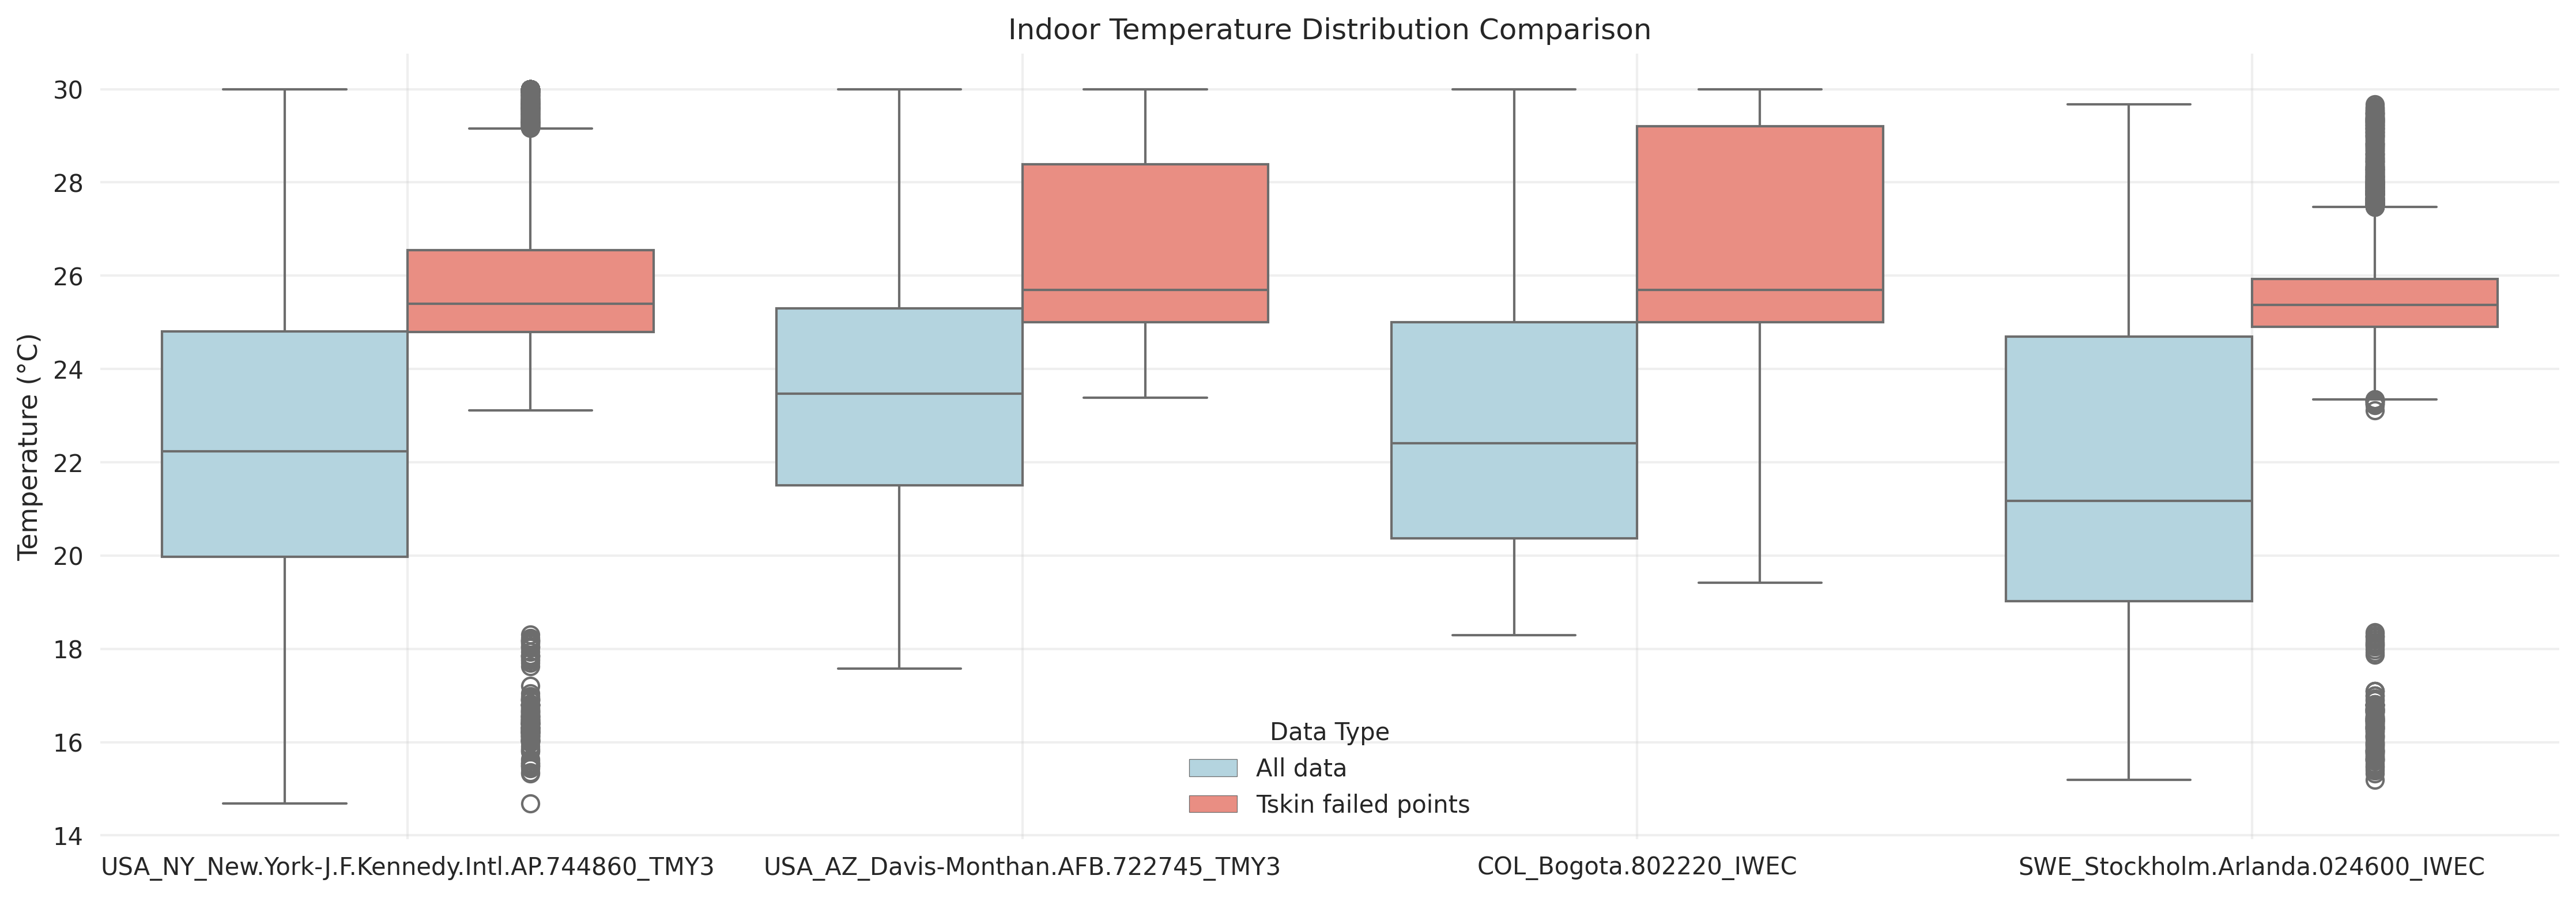
\includegraphics[width=0.75\linewidth]{figs/temp_distribution_comparison.png}
    \caption{Comparison of the air temperature distribution across all data points and the subset of instances where the $T_{skin}$ condition was not met with \texttt{pv-tsk-strict} mode}
    \label{fig:tsk_ta_distribution}
\end{figure}

Incorporating physiological metrics such as $T_{skin}$ into HVAC control logic significantly enhanced occupant comfort with minimal additional energy consumption. This result emphasizes the promising potential of physiology-informed control strategies to transform conventional building management approaches.



\subsection{Robustness Under Stochastic Weather Conditions}
The use of stochastic weather perturbations throughout our simulations provides inherent validation of our findings' statistical robustness. Despite random variations of $\pm$2.5$^\circ$C (1$\sigma$) applied to temperature readings at each 15-minute timestep—equivalent to sensor uncertainty and microclimate variations in real buildings—the performance hierarchy remains remarkably stable:
\begin{itemize}
    \item Grid-search optimized variants (pmv-o, lightgbm-o, pv-o) consistently rank in the top three positions across all climates
    \item Energy savings percentages show low variance: optimized PMV achieves 15-18.5\% savings with less than $\pm$2\% variation across weather realizations
    \item Comfort metrics remain stable: median PMV stays within $\pm$0.1 of target despite weather perturbations
\end{itemize}

This stability under stochastic conditions demonstrates that our findings are not artifacts of specific weather patterns but represent fundamental differences in control strategy effectiveness. The consistent performance gaps between optimized and naive controllers across thousands of unique weather realizations provide strong statistical evidence for our conclusions without requiring extensive Monte Carlo studies.